\chapter{Phase 1 - Uniform Bonding}

\section{Process}
The process in this section will aim to first characterize the spread of indium over the surface \ref{sec:indiumSpread} of the `LED' and `backplane' (`BP') substrates
\footnote{The LED and backplane are in quotes as these are not actual LEDs or backplanes with transistors, but instead are mock samples with similar physical characteristics.
Those characteristics being the sample size and the $\ch{In}-\ch{Au}$ coating on the samples.
Differences arise from the lack of a MESA structure that will be seen in the successive chapter
\ref{sec:BondingToLEDS}}
and secondly validate uniform bonding over the surface of the sample \ref{sec:uniformBond}.

The process that will be used to explore this is the following.
\begin{enumerate}
    \item Electroplate indium onto a `BP'
    \item Remove photoresist from sample with Acetone then IPA rinse or Remover PG (follow the instructions in \cite{RemoverPGds})
    \item Do surface activation of LED and BP using the plasma cleaner
    \item Place BP face up and LED face down on diebonder
    \item Using Pick-And-Place (P+P) function on diebonder, pick the LED and place on the BP using the specified bonding pressure and heat recipe
    \begin{description}
        \item[Bonder Head] Ensure that the bond head being used is a gimbal bond head \footnote{Gimbal diebonding head is used to minimize non-uniformity of bonding pressure over the surface of the sample}
        \item[P+P] The recipe used on the diebonder for P+P is as following: \begin{itemize}
            \item Approach and lift the LED using the vacuum function with an application force of $30\unit{\gram}$
            \item Complete translational and axial alignment of the LEDs to the BP using the flip-chip camera \footnote{Due to the limitations of the diebonder in the packaging lab, alignment must be done on only one section of the viewfinder. This is due to the non-planar alignment of the optical path in the flip-chip camera.}
            \item Ensure the eutectic bonding module is on and set to a place force of $3\unit{\kilo\gram}$
            \item Load the correct recipe: $10\unit{\second} \text{@} 60\dC$ followed by $3\unit{\minute} \text{@} 250\dC$
        \end{itemize}
    \end{description}
\end{enumerate}

After a repeatable electroplating process for indium was developed, the next step was to investigate how the indium would spread once die-bonded. The spreading behaviour of indium is critical because it can impact the performance of the semiconductor device. Specifically, the spreading of indium can affect the heat dissipation and the electrical contact between the die and the substrate. Understanding this behaviour is essential for optimizing the performance of the device.
This knowledge can then be used to inform the design and manufacture of semiconductor devices, improving their reliability and performance.
Diebonding is the process of placing a semiconductor chip onto a substrate or package, and eutectic bonding is a common diebonding technique. Understanding the behaviour of indium during eutectic bonding is crucial for ensuring the reliability and performance of the final device.

A flipchip diebonder is a machine that is used to bond microelectronic chips directly onto a substrate. It allows for precise alignment and bonding of the chip to the substrate, which is essential for the proper functioning of microelectronic devices. In addition to the standard bonding techniques, a flipchip diebonder with eutectic bonding capabilities enables the bonding of two chips by bonding with precise control of heat and pressure, which can greatly enhance the reliability and performance of the microelectronic device. Eutectic bonding is a specialized technique that involves heating the two materials to their eutectic point, at which they melt and fuse together, creating a bond. \footnote{The material and strength properties of the bond will be discussed further in the chapter in section \ref{sec:Ch2_repeatable}} This makes the flipchip diebonder with eutectic bonding capability a valuable tool in the field of microelectronics for high-performance and reliable bonding of chips to substrates.


The diebonder being used is the `TRESKY-diebond' tool in the QNC packaging lab it is the Tresky T-3000-FC3 model.
The tool is capable of providing a bonding force of up to $490 \unit{\newton}$ ($50 \unit{\kg}$ mass) may be applied at temperatures up to $400 \dC$. The datasheet suggests that it offers placement accuracy of $\pm10\um$ \cite{diebonderDatasheet}, While not specified, there are also inherent limitations to the axial accuracy due to the backlash in the gearing of the rotational alignment system.



\section{Characterization of Indium Bonding Spread}
\label{sec:indiumSpread}

In this section, we will explore the characterization of indium spreading during the diebonding process. The primary goal is to gain a deeper understanding of how the indium will melt and spread during the process. We will achieve this by analyzing SEM images of the initial volume and microscope images taken after diebonding. Through this analysis, we aim to identify and quantify the parameters that influence indium spreading and develop an understanding of the fundamental mechanisms involved. The insights gained from this section will help optimize the diebonding process and improve the quality of the final product.

When indium is deposited on a substrate, it forms cylindrical columns that are circular when viewed from the top. During the diebonding process, the indium will melt and spread to form a bond between the substrate and the die. We expect the indium to spread in a circular fashion due to the surface tension of the liquid metal and due to the physical constraints for the material to move when being in essence `squeezed' between two plates. As the indium melts, its surface will try to minimize its surface area and form a shape with the lowest surface area possible, which in this case is a circle. Therefore, understanding the spreading behaviour of the indium is crucial for achieving a successful diebonding process.

Since we want to calculate and understand how the indium will conform when bonding is done, a number of characterization measurements were conducted to understand how the indium will spread and expand over the sample surface. We know the volume of indium will not change when diebonding occurs, we can model the spread of indium as a flattening of a cylinder.

\begin{equation} \label{eq:radius_indium}
    \begin{split}
        V_{Cylinder Initial} &= V_{Cylinder Final} \\
        \pi \times r_{Initial}^2 \times h_{Initial} &= \pi \times r_{Final}^2 \times h_{Final} \\
        \sqrt{\frac{h_{Initial}}{h_{Final}}} r_{Initial} &= r_{Final} \\
        \sqrt{\frac{h_{Initial}}{ 0.65 \um}} r_{Initial} &= r_{Final}
    \end{split}
\end{equation}


\begin{figure}
    \centering
\begin{subfigure}[t]{0.3\textwidth}
    \centering
    \tiny
    \begin{tikzpicture}
        % define cell size
        \def\cSz{0.4cm}
        \def\N{12}

        % draw table border
        \draw (0,0) rectangle (\N*\cSz,\N*\cSz);

        \foreach \x in {1,2,3,4,5,6,7,8,9,10,11} {
            % draw horizontal lines
            \draw (0,\x*\cSz) -- (\N*\cSz,\x*\cSz);
            % draw vertical lines
            \draw (\x*\cSz,0) -- (\x*\cSz,\N*\cSz);
        }
        % add cell contents
        \draw[fill=purple4!28.3, draw] (0.0 * \cSz, 0.0 * \cSz) rectangle (1.0 * \cSz, 1.0 * \cSz);
\node at (0.5 * \cSz, 0.5 * \cSz)  { 4.80 };
\draw[fill=purple4!32.2, draw] (0.0 * \cSz, 2.0 * \cSz) rectangle (1.0 * \cSz, 3.0 * \cSz);
\node at (0.5 * \cSz, 2.5 * \cSz)  { 5.22 };
\draw[fill=purple4!19.6, draw] (0.0 * \cSz, 5.0 * \cSz) rectangle (1.0 * \cSz, 6.0 * \cSz);
\node at (0.5 * \cSz, 5.5 * \cSz)  { 3.98 };
\draw[fill=purple4!20.4, draw] (0.0 * \cSz, 6.0 * \cSz) rectangle (1.0 * \cSz, 7.0 * \cSz);
\node at (0.5 * \cSz, 6.5 * \cSz)  { 4.05 };
\draw[fill=purple4!33.1, draw] (0.0 * \cSz, 9.0 * \cSz) rectangle (1.0 * \cSz, 10.0 * \cSz);
\node at (0.5 * \cSz, 9.5 * \cSz)  { 5.32 };
\draw[fill=purple4!33.2, draw] (0.0 * \cSz, 11.0 * \cSz) rectangle (1.0 * \cSz, 12.0 * \cSz);
\node at (0.5 * \cSz, 11.5 * \cSz)  { 5.33     };
\draw[fill=purple4!11.3, draw] (2.0 * \cSz, 5.0 * \cSz) rectangle (3.0 * \cSz, 6.0 * \cSz);
\node at (2.5 * \cSz, 5.5 * \cSz)  { 3.33 };
\draw[fill=purple4!28.8, draw] (2.0 * \cSz, 6.0 * \cSz) rectangle (3.0 * \cSz, 7.0 * \cSz);
\node at (2.5 * \cSz, 6.5 * \cSz)  { 4.85 };
\draw[fill=purple4!0.0, draw] (3.0 * \cSz, 0.0 * \cSz) rectangle (4.0 * \cSz, 1.0 * \cSz);
\node at (3.5 * \cSz, 0.5 * \cSz)  { 2.61 };
\draw[fill=purple4!9.2, draw] (3.0 * \cSz, 3.0 * \cSz) rectangle (4.0 * \cSz, 4.0 * \cSz);
\node at (3.5 * \cSz, 3.5 * \cSz)  { 3.18 };
\draw[fill=purple4!28.4, draw] (3.0 * \cSz, 8.0 * \cSz) rectangle (4.0 * \cSz, 9.0 * \cSz);
\node at (3.5 * \cSz, 8.5 * \cSz)  { 4.81 };
\draw[fill=purple4!33.8, draw] (3.0 * \cSz, 11.0 * \cSz) rectangle (4.0 * \cSz, 12.0 * \cSz);
\node at (3.5 * \cSz, 11.5 * \cSz)  { 5.40     };
\draw[fill=purple4!6.8, draw] (5.0 * \cSz, 0.0 * \cSz) rectangle (6.0 * \cSz, 1.0 * \cSz);
\node at (5.5 * \cSz, 0.5 * \cSz)  { 3.02 };
\draw[fill=purple4!8.1, draw] (5.0 * \cSz, 2.0 * \cSz) rectangle (6.0 * \cSz, 3.0 * \cSz);
\node at (5.5 * \cSz, 2.5 * \cSz)  { 3.11 };
\draw[fill=purple4!18.4, draw] (5.0 * \cSz, 5.0 * \cSz) rectangle (6.0 * \cSz, 6.0 * \cSz);
\node at (5.5 * \cSz, 5.5 * \cSz)  { 3.88 };
\draw[fill=purple4!32.8, draw] (5.0 * \cSz, 6.0 * \cSz) rectangle (6.0 * \cSz, 7.0 * \cSz);
\node at (5.5 * \cSz, 6.5 * \cSz)  { 5.29 };
\draw[fill=purple4!17.2, draw] (5.0 * \cSz, 9.0 * \cSz) rectangle (6.0 * \cSz, 10.0 * \cSz);
\node at (5.5 * \cSz, 9.5 * \cSz)  { 3.78 };
\draw[fill=purple4!18.4, draw] (5.0 * \cSz, 11.0 * \cSz) rectangle (6.0 * \cSz, 12.0 * \cSz);
\node at (5.5 * \cSz, 11.5 * \cSz)  { 3.88     };
\draw[fill=purple4!42.8, draw] (6.0 * \cSz, 0.0 * \cSz) rectangle (7.0 * \cSz, 1.0 * \cSz);
\node at (6.5 * \cSz, 0.5 * \cSz)  { 6.55 };
\draw[fill=purple4!70.9, draw] (6.0 * \cSz, 2.0 * \cSz) rectangle (7.0 * \cSz, 3.0 * \cSz);
\node at (6.5 * \cSz, 2.5 * \cSz)  { 12.0 };
\draw[fill=purple4!90.0, draw] (6.0 * \cSz, 5.0 * \cSz) rectangle (7.0 * \cSz, 6.0 * \cSz);
\node at (6.5 * \cSz, 5.5 * \cSz)  { 18.1 };
\draw[fill=purple4!29.7, draw] (6.0 * \cSz, 6.0 * \cSz) rectangle (7.0 * \cSz, 7.0 * \cSz);
\node at (6.5 * \cSz, 6.5 * \cSz)  { 4.94 };
\draw[fill=purple4!25.8, draw] (6.0 * \cSz, 9.0 * \cSz) rectangle (7.0 * \cSz, 10.0 * \cSz);
\node at (6.5 * \cSz, 9.5 * \cSz)  { 4.55 };
\draw[fill=purple4!30.3, draw] (6.0 * \cSz, 11.0 * \cSz) rectangle (7.0 * \cSz, 12.0 * \cSz);
\node at (6.5 * \cSz, 11.5 * \cSz)  { 5.01     };
\draw[fill=purple4!39.8, draw] (8.0 * \cSz, 0.0 * \cSz) rectangle (9.0 * \cSz, 1.0 * \cSz);
\node at (8.5 * \cSz, 0.5 * \cSz)  { 6.15 };
\draw[fill=purple4!40.8, draw] (8.0 * \cSz, 3.0 * \cSz) rectangle (9.0 * \cSz, 4.0 * \cSz);
\node at (8.5 * \cSz, 3.5 * \cSz)  { 6.28 };
\draw[fill=purple4!56.6, draw] (8.0 * \cSz, 5.0 * \cSz) rectangle (9.0 * \cSz, 6.0 * \cSz);
\node at (8.5 * \cSz, 5.5 * \cSz)  { 8.82 };
\draw[fill=purple4!39.0, draw] (8.0 * \cSz, 11.0 * \cSz) rectangle (9.0 * \cSz, 12.0 * \cSz);
\node at (8.5 * \cSz, 11.5 * \cSz)  { 6.04     };
\draw[fill=purple4!29.7, draw] (9.0 * \cSz, 6.0 * \cSz) rectangle (10.0 * \cSz, 7.0 * \cSz);
\node at (9.5 * \cSz, 6.5 * \cSz)  { 4.95 };
\draw[fill=purple4!27.0, draw] (9.0 * \cSz, 9.0 * \cSz) rectangle (10.0 * \cSz, 10.0 * \cSz);
\node at (9.5 * \cSz, 9.5 * \cSz)  { 4.67 };
\draw[fill=purple4!40.3, draw] (11.0 * \cSz, 0.0 * \cSz) rectangle (12.0 * \cSz, 1.0 * \cSz);
\node at (11.5 * \cSz, 0.5 * \cSz)  { 6.21 };
\draw[fill=purple4!67.3, draw] (11.0 * \cSz, 2.0 * \cSz) rectangle (12.0 * \cSz, 3.0 * \cSz);
\node at (11.5 * \cSz, 2.5 * \cSz)  { 11.1 };
\draw[fill=purple4!55.3, draw] (11.0 * \cSz, 5.0 * \cSz) rectangle (12.0 * \cSz, 6.0 * \cSz);
\node at (11.5 * \cSz, 5.5 * \cSz)  { 8.57 };
\draw[fill=purple4!30.9, draw] (11.0 * \cSz, 6.0 * \cSz) rectangle (12.0 * \cSz, 7.0 * \cSz);
\node at (11.5 * \cSz, 6.5 * \cSz)  { 5.08 };
\draw[fill=purple4!35.0, draw] (11.0 * \cSz, 9.0 * \cSz) rectangle (12.0 * \cSz, 10.0 * \cSz);
\node at (11.5 * \cSz, 9.5 * \cSz)  { 5.54 };
\draw[fill=purple4!38.6, draw] (11.0 * \cSz, 11.0 * \cSz) rectangle (12.0 * \cSz, 12.0 * \cSz);
\node at (11.5 * \cSz, 11.5 * \cSz)  { 5.99     };


    \end{tikzpicture}
    \caption{Indium bump height map. Saturation of colour indicates relative thickness.}
    \label{fig:bumpHeightMap}
\end{subfigure}
~
\begin{subfigure}[t]{0.3\textwidth}
    \centering
    \tiny
    \begin{tikzpicture}
        % define cell size
        \def\cSz{0.4cm}
        \def\N{12}

        % draw table border
        \draw (0,0) rectangle (\N*\cSz,\N*\cSz);

        \foreach \x in {1,2,3,4,5,6,7,8,9,10,11} {
            % draw horizontal lines
            \draw (0,\x*\cSz) -- (\N*\cSz,\x*\cSz);
            % draw vertical lines
            \draw (\x*\cSz,0) -- (\x*\cSz,\N*\cSz);
        }
        % add cell contents
        \draw[fill=purple4!16.0, draw] (0.0 * \cSz, 0.0 * \cSz) rectangle (1.0 * \cSz, 1.0 * \cSz);
\node at (0.5 * \cSz, 0.5 * \cSz)  { 16.4 };
\draw[fill=purple4!37.8, draw] (0.0 * \cSz, 2.0 * \cSz) rectangle (1.0 * \cSz, 3.0 * \cSz);
\node at (0.5 * \cSz, 2.5 * \cSz)  { 18.7 };
\draw[fill=purple4!17.0, draw] (0.0 * \cSz, 5.0 * \cSz) rectangle (1.0 * \cSz, 6.0 * \cSz);
\node at (0.5 * \cSz, 5.5 * \cSz)  { 16.5 };
\draw[fill=purple4!12.9, draw] (0.0 * \cSz, 6.0 * \cSz) rectangle (1.0 * \cSz, 7.0 * \cSz);
\node at (0.5 * \cSz, 6.5 * \cSz)  { 16.1 };
\draw[fill=purple4!17.0, draw] (0.0 * \cSz, 9.0 * \cSz) rectangle (1.0 * \cSz, 10.0 * \cSz);
\node at (0.5 * \cSz, 9.5 * \cSz)  { 16.5 };
\draw[fill=purple4!11.8, draw] (0.0 * \cSz, 11.0 * \cSz) rectangle (1.0 * \cSz, 12.0 * \cSz);
\node at (0.5 * \cSz, 11.5 * \cSz)  { 16.0     };
\draw[fill=purple4!12.9, draw] (2.0 * \cSz, 5.0 * \cSz) rectangle (3.0 * \cSz, 6.0 * \cSz);
\node at (2.5 * \cSz, 5.5 * \cSz)  { 16.1 };
\draw[fill=purple4!11.8, draw] (2.0 * \cSz, 6.0 * \cSz) rectangle (3.0 * \cSz, 7.0 * \cSz);
\node at (2.5 * \cSz, 6.5 * \cSz)  { 16.0 };
\draw[fill=purple4!22.9, draw] (3.0 * \cSz, 0.0 * \cSz) rectangle (4.0 * \cSz, 1.0 * \cSz);
\node at (3.5 * \cSz, 0.5 * \cSz)  { 17.1 };
\draw[fill=purple4!14.9, draw] (3.0 * \cSz, 3.0 * \cSz) rectangle (4.0 * \cSz, 4.0 * \cSz);
\node at (3.5 * \cSz, 3.5 * \cSz)  { 16.3 };
\draw[fill=purple4!5.5, draw] (3.0 * \cSz, 8.0 * \cSz) rectangle (4.0 * \cSz, 9.0 * \cSz);
\node at (3.5 * \cSz, 8.5 * \cSz)  { 15.4 };
\draw[fill=purple4!10.8, draw] (3.0 * \cSz, 11.0 * \cSz) rectangle (4.0 * \cSz, 12.0 * \cSz);
\node at (3.5 * \cSz, 11.5 * \cSz)  { 15.9     };
\draw[fill=purple4!21.9, draw] (5.0 * \cSz, 0.0 * \cSz) rectangle (6.0 * \cSz, 1.0 * \cSz);
\node at (5.5 * \cSz, 0.5 * \cSz)  { 17.0 };
\draw[fill=purple4!19.0, draw] (5.0 * \cSz, 2.0 * \cSz) rectangle (6.0 * \cSz, 3.0 * \cSz);
\node at (5.5 * \cSz, 2.5 * \cSz)  { 16.7 };
\draw[fill=purple4!7.6, draw] (5.0 * \cSz, 5.0 * \cSz) rectangle (6.0 * \cSz, 6.0 * \cSz);
\node at (5.5 * \cSz, 5.5 * \cSz)  { 15.6 };
\draw[fill=purple4!14.9, draw] (5.0 * \cSz, 6.0 * \cSz) rectangle (6.0 * \cSz, 7.0 * \cSz);
\node at (5.5 * \cSz, 6.5 * \cSz)  { 16.3 };
\draw[fill=purple4!5.5, draw] (5.0 * \cSz, 9.0 * \cSz) rectangle (6.0 * \cSz, 10.0 * \cSz);
\node at (5.5 * \cSz, 9.5 * \cSz)  { 15.4 };
\draw[fill=purple4!9.8, draw] (5.0 * \cSz, 11.0 * \cSz) rectangle (6.0 * \cSz, 12.0 * \cSz);
\node at (5.5 * \cSz, 11.5 * \cSz)  { 15.8     };
\draw[fill=purple4!0.0, draw] (6.0 * \cSz, 0.0 * \cSz) rectangle (7.0 * \cSz, 1.0 * \cSz);
\node at (6.5 * \cSz, 0.5 * \cSz)  { 14.9 };
\draw[fill=purple4!63.3, draw] (6.0 * \cSz, 2.0 * \cSz) rectangle (7.0 * \cSz, 3.0 * \cSz);
\node at (6.5 * \cSz, 2.5 * \cSz)  { 21.8 };
\draw[fill=purple4!90.0, draw] (6.0 * \cSz, 5.0 * \cSz) rectangle (7.0 * \cSz, 6.0 * \cSz);
\node at (6.5 * \cSz, 5.5 * \cSz)  { 25.6 };
\draw[fill=purple4!31.4, draw] (6.0 * \cSz, 6.0 * \cSz) rectangle (7.0 * \cSz, 7.0 * \cSz);
\node at (6.5 * \cSz, 6.5 * \cSz)  { 18.0 };
\draw[fill=purple4!44.7, draw] (6.0 * \cSz, 9.0 * \cSz) rectangle (7.0 * \cSz, 10.0 * \cSz);
\node at (6.5 * \cSz, 9.5 * \cSz)  { 19.5 };
\draw[fill=purple4!27.7, draw] (6.0 * \cSz, 11.0 * \cSz) rectangle (7.0 * \cSz, 12.0 * \cSz);
\node at (6.5 * \cSz, 11.5 * \cSz)  { 17.6     };
\draw[fill=purple4!46.4, draw] (8.0 * \cSz, 0.0 * \cSz) rectangle (9.0 * \cSz, 1.0 * \cSz);
\node at (8.5 * \cSz, 0.5 * \cSz)  { 19.7 };
\draw[fill=purple4!43.0, draw] (8.0 * \cSz, 3.0 * \cSz) rectangle (9.0 * \cSz, 4.0 * \cSz);
\node at (8.5 * \cSz, 3.5 * \cSz)  { 19.3 };
\draw[fill=purple4!55.5, draw] (8.0 * \cSz, 5.0 * \cSz) rectangle (9.0 * \cSz, 6.0 * \cSz);
\node at (8.5 * \cSz, 5.5 * \cSz)  { 20.8 };
\draw[fill=purple4!46.4, draw] (8.0 * \cSz, 11.0 * \cSz) rectangle (9.0 * \cSz, 12.0 * \cSz);
\node at (8.5 * \cSz, 11.5 * \cSz)  { 19.7     };
\draw[fill=purple4!37.8, draw] (9.0 * \cSz, 6.0 * \cSz) rectangle (10.0 * \cSz, 7.0 * \cSz);
\node at (9.5 * \cSz, 6.5 * \cSz)  { 18.7 };
\draw[fill=purple4!44.7, draw] (9.0 * \cSz, 9.0 * \cSz) rectangle (10.0 * \cSz, 10.0 * \cSz);
\node at (9.5 * \cSz, 9.5 * \cSz)  { 19.5 };
\draw[fill=purple4!52.2, draw] (11.0 * \cSz, 0.0 * \cSz) rectangle (12.0 * \cSz, 1.0 * \cSz);
\node at (11.5 * \cSz, 0.5 * \cSz)  { 20.4 };
\draw[fill=purple4!63.3, draw] (11.0 * \cSz, 2.0 * \cSz) rectangle (12.0 * \cSz, 3.0 * \cSz);
\node at (11.5 * \cSz, 2.5 * \cSz)  { 21.8 };
\draw[fill=purple4!23.9, draw] (11.0 * \cSz, 5.0 * \cSz) rectangle (12.0 * \cSz, 6.0 * \cSz);
\node at (11.5 * \cSz, 5.5 * \cSz)  { 17.2 };
\draw[fill=purple4!49.8, draw] (11.0 * \cSz, 6.0 * \cSz) rectangle (12.0 * \cSz, 7.0 * \cSz);
\node at (11.5 * \cSz, 6.5 * \cSz)  { 20.1 };
\draw[fill=purple4!66.3, draw] (11.0 * \cSz, 9.0 * \cSz) rectangle (12.0 * \cSz, 10.0 * \cSz);
\node at (11.5 * \cSz, 9.5 * \cSz)  { 22.2 };
\draw[fill=purple4!60.2, draw] (11.0 * \cSz, 11.0 * \cSz) rectangle (12.0 * \cSz, 12.0 * \cSz);
\node at (11.5 * \cSz, 11.5 * \cSz)  { 21.4     };


    \end{tikzpicture}
    \caption{Indium bump width map. Saturation of colour indicates relative width.}
    \label{fig:bumpWidthMap}
\end{subfigure}
~
\begin{subfigure}[t]{0.3\textwidth}
    \centering
    \tiny
    \begin{tikzpicture}
        % define cell size
        \def\cSz{0.4cm}
        \def\N{12}

        % draw table border
        \draw (0,0) rectangle (\N*\cSz,\N*\cSz);

        \foreach \x in {1,2,3,4,5,6,7,8,9,10,11} {
            % draw horizontal lines
            \draw (0,\x*\cSz) -- (\N*\cSz,\x*\cSz);
            % draw vertical lines
            \draw (\x*\cSz,0) -- (\x*\cSz,\N*\cSz);
        }
        % add cell contents
        \draw[fill=purple4!17.3, draw] (0.0 * \cSz, 0.0 * \cSz) rectangle (1.0 * \cSz, 1.0 * \cSz);
\node at (0.5 * \cSz, 0.5 * \cSz)  { 1014 };
\draw[fill=purple4!28.6, draw] (0.0 * \cSz, 2.0 * \cSz) rectangle (1.0 * \cSz, 3.0 * \cSz);
\node at (0.5 * \cSz, 2.5 * \cSz)  { 1434 };
\draw[fill=purple4!11.5, draw] (0.0 * \cSz, 5.0 * \cSz) rectangle (1.0 * \cSz, 6.0 * \cSz);
\node at (0.5 * \cSz, 5.5 * \cSz)  {  851 };
\draw[fill=purple4!10.3, draw] (0.0 * \cSz, 6.0 * \cSz) rectangle (1.0 * \cSz, 7.0 * \cSz);
\node at (0.5 * \cSz, 6.5 * \cSz)  {  819 };
\draw[fill=purple4!20.8, draw] (0.0 * \cSz, 9.0 * \cSz) rectangle (1.0 * \cSz, 10.0 * \cSz);
\node at (0.5 * \cSz, 9.5 * \cSz)  { 1131 };
\draw[fill=purple4!19.1, draw] (0.0 * \cSz, 11.0 * \cSz) rectangle (1.0 * \cSz, 12.0 * \cSz);
\node at (0.5 * \cSz, 11.5 * \cSz)  { 1072         };
\draw[fill=purple4!4.1, draw] (2.0 * \cSz, 5.0 * \cSz) rectangle (3.0 * \cSz, 6.0 * \cSz);
\node at (2.5 * \cSz, 5.5 * \cSz)  {  678 };
\draw[fill=purple4!16.0, draw] (2.0 * \cSz, 6.0 * \cSz) rectangle (3.0 * \cSz, 7.0 * \cSz);
\node at (2.5 * \cSz, 6.5 * \cSz)  {  975 };
\draw[fill=purple4!0.0, draw] (3.0 * \cSz, 0.0 * \cSz) rectangle (4.0 * \cSz, 1.0 * \cSz);
\node at (3.5 * \cSz, 0.5 * \cSz)  {  599 };
\draw[fill=purple4!3.4, draw] (3.0 * \cSz, 3.0 * \cSz) rectangle (4.0 * \cSz, 4.0 * \cSz);
\node at (3.5 * \cSz, 3.5 * \cSz)  {  664 };
\draw[fill=purple4!13.2, draw] (3.0 * \cSz, 8.0 * \cSz) rectangle (4.0 * \cSz, 9.0 * \cSz);
\node at (3.5 * \cSz, 8.5 * \cSz)  {  896 };
\draw[fill=purple4!18.9, draw] (3.0 * \cSz, 11.0 * \cSz) rectangle (4.0 * \cSz, 12.0 * \cSz);
\node at (3.5 * \cSz, 11.5 * \cSz)  { 1065         };
\draw[fill=purple4!4.4, draw] (5.0 * \cSz, 0.0 * \cSz) rectangle (6.0 * \cSz, 1.0 * \cSz);
\node at (5.5 * \cSz, 0.5 * \cSz)  {  685 };
\draw[fill=purple4!4.2, draw] (5.0 * \cSz, 2.0 * \cSz) rectangle (6.0 * \cSz, 3.0 * \cSz);
\node at (5.5 * \cSz, 2.5 * \cSz)  {  681 };
\draw[fill=purple4!7.0, draw] (5.0 * \cSz, 5.0 * \cSz) rectangle (6.0 * \cSz, 6.0 * \cSz);
\node at (5.5 * \cSz, 5.5 * \cSz)  {  742 };
\draw[fill=purple4!19.8, draw] (5.0 * \cSz, 6.0 * \cSz) rectangle (6.0 * \cSz, 7.0 * \cSz);
\node at (5.5 * \cSz, 6.5 * \cSz)  { 1097 };
\draw[fill=purple4!5.3, draw] (5.0 * \cSz, 9.0 * \cSz) rectangle (6.0 * \cSz, 10.0 * \cSz);
\node at (5.5 * \cSz, 9.5 * \cSz)  {  704 };
\draw[fill=purple4!7.9, draw] (5.0 * \cSz, 11.0 * \cSz) rectangle (6.0 * \cSz, 12.0 * \cSz);
\node at (5.5 * \cSz, 11.5 * \cSz)  {  761         };
\draw[fill=purple4!21.2, draw] (6.0 * \cSz, 0.0 * \cSz) rectangle (7.0 * \cSz, 1.0 * \cSz);
\node at (6.5 * \cSz, 0.5 * \cSz)  { 1142 };
\draw[fill=purple4!66.0, draw] (6.0 * \cSz, 2.0 * \cSz) rectangle (7.0 * \cSz, 3.0 * \cSz);
\node at (6.5 * \cSz, 2.5 * \cSz)  { 4479 };
\draw[fill=purple4!90.0, draw] (6.0 * \cSz, 5.0 * \cSz) rectangle (7.0 * \cSz, 6.0 * \cSz);
\node at (6.5 * \cSz, 5.5 * \cSz)  { 9316 };
\draw[fill=purple4!24.3, draw] (6.0 * \cSz, 6.0 * \cSz) rectangle (7.0 * \cSz, 7.0 * \cSz);
\node at (6.5 * \cSz, 6.5 * \cSz)  { 1257 };
\draw[fill=purple4!26.7, draw] (6.0 * \cSz, 9.0 * \cSz) rectangle (7.0 * \cSz, 10.0 * \cSz);
\node at (6.5 * \cSz, 9.5 * \cSz)  { 1352 };
\draw[fill=purple4!23.1, draw] (6.0 * \cSz, 11.0 * \cSz) rectangle (7.0 * \cSz, 12.0 * \cSz);
\node at (6.5 * \cSz, 11.5 * \cSz)  { 1212         };
\draw[fill=purple4!37.4, draw] (8.0 * \cSz, 0.0 * \cSz) rectangle (9.0 * \cSz, 1.0 * \cSz);
\node at (8.5 * \cSz, 0.5 * \cSz)  { 1875 };
\draw[fill=purple4!36.6, draw] (8.0 * \cSz, 3.0 * \cSz) rectangle (9.0 * \cSz, 4.0 * \cSz);
\node at (8.5 * \cSz, 3.5 * \cSz)  { 1828 };
\draw[fill=purple4!52.8, draw] (8.0 * \cSz, 5.0 * \cSz) rectangle (9.0 * \cSz, 6.0 * \cSz);
\node at (8.5 * \cSz, 5.5 * \cSz)  { 2995 };
\draw[fill=purple4!36.7, draw] (8.0 * \cSz, 11.0 * \cSz) rectangle (9.0 * \cSz, 12.0 * \cSz);
\node at (8.5 * \cSz, 11.5 * \cSz)  { 1832         };
\draw[fill=purple4!26.9, draw] (9.0 * \cSz, 6.0 * \cSz) rectangle (10.0 * \cSz, 7.0 * \cSz);
\node at (9.5 * \cSz, 6.5 * \cSz)  { 1359 };
\draw[fill=purple4!27.7, draw] (9.0 * \cSz, 9.0 * \cSz) rectangle (10.0 * \cSz, 10.0 * \cSz);
\node at (9.5 * \cSz, 9.5 * \cSz)  { 1395 };
\draw[fill=purple4!40.0, draw] (11.0 * \cSz, 0.0 * \cSz) rectangle (12.0 * \cSz, 1.0 * \cSz);
\node at (11.5 * \cSz, 0.5 * \cSz)  { 2030 };
\draw[fill=purple4!63.4, draw] (11.0 * \cSz, 2.0 * \cSz) rectangle (12.0 * \cSz, 3.0 * \cSz);
\node at (11.5 * \cSz, 2.5 * \cSz)  { 4145 };
\draw[fill=purple4!39.2, draw] (11.0 * \cSz, 5.0 * \cSz) rectangle (12.0 * \cSz, 6.0 * \cSz);
\node at (11.5 * \cSz, 5.5 * \cSz)  { 1979 };
\draw[fill=purple4!32.3, draw] (11.0 * \cSz, 6.0 * \cSz) rectangle (12.0 * \cSz, 7.0 * \cSz);
\node at (11.5 * \cSz, 6.5 * \cSz)  { 1604 };
\draw[fill=purple4!41.7, draw] (11.0 * \cSz, 9.0 * \cSz) rectangle (12.0 * \cSz, 10.0 * \cSz);
\node at (11.5 * \cSz, 9.5 * \cSz)  { 2135 };
\draw[fill=purple4!41.8, draw] (11.0 * \cSz, 11.0 * \cSz) rectangle (12.0 * \cSz, 12.0 * \cSz);
\node at (11.5 * \cSz, 11.5 * \cSz)  { 2144         };


    \end{tikzpicture}
    \caption{Indium bump volume map. Saturation of colour indicates relative volume.}
    \label{fig:bumpVolumeMap}
\end{subfigure}
\caption{Maps of indium bump metrics.}
\end{figure}

\begin{figure}
    \centering
    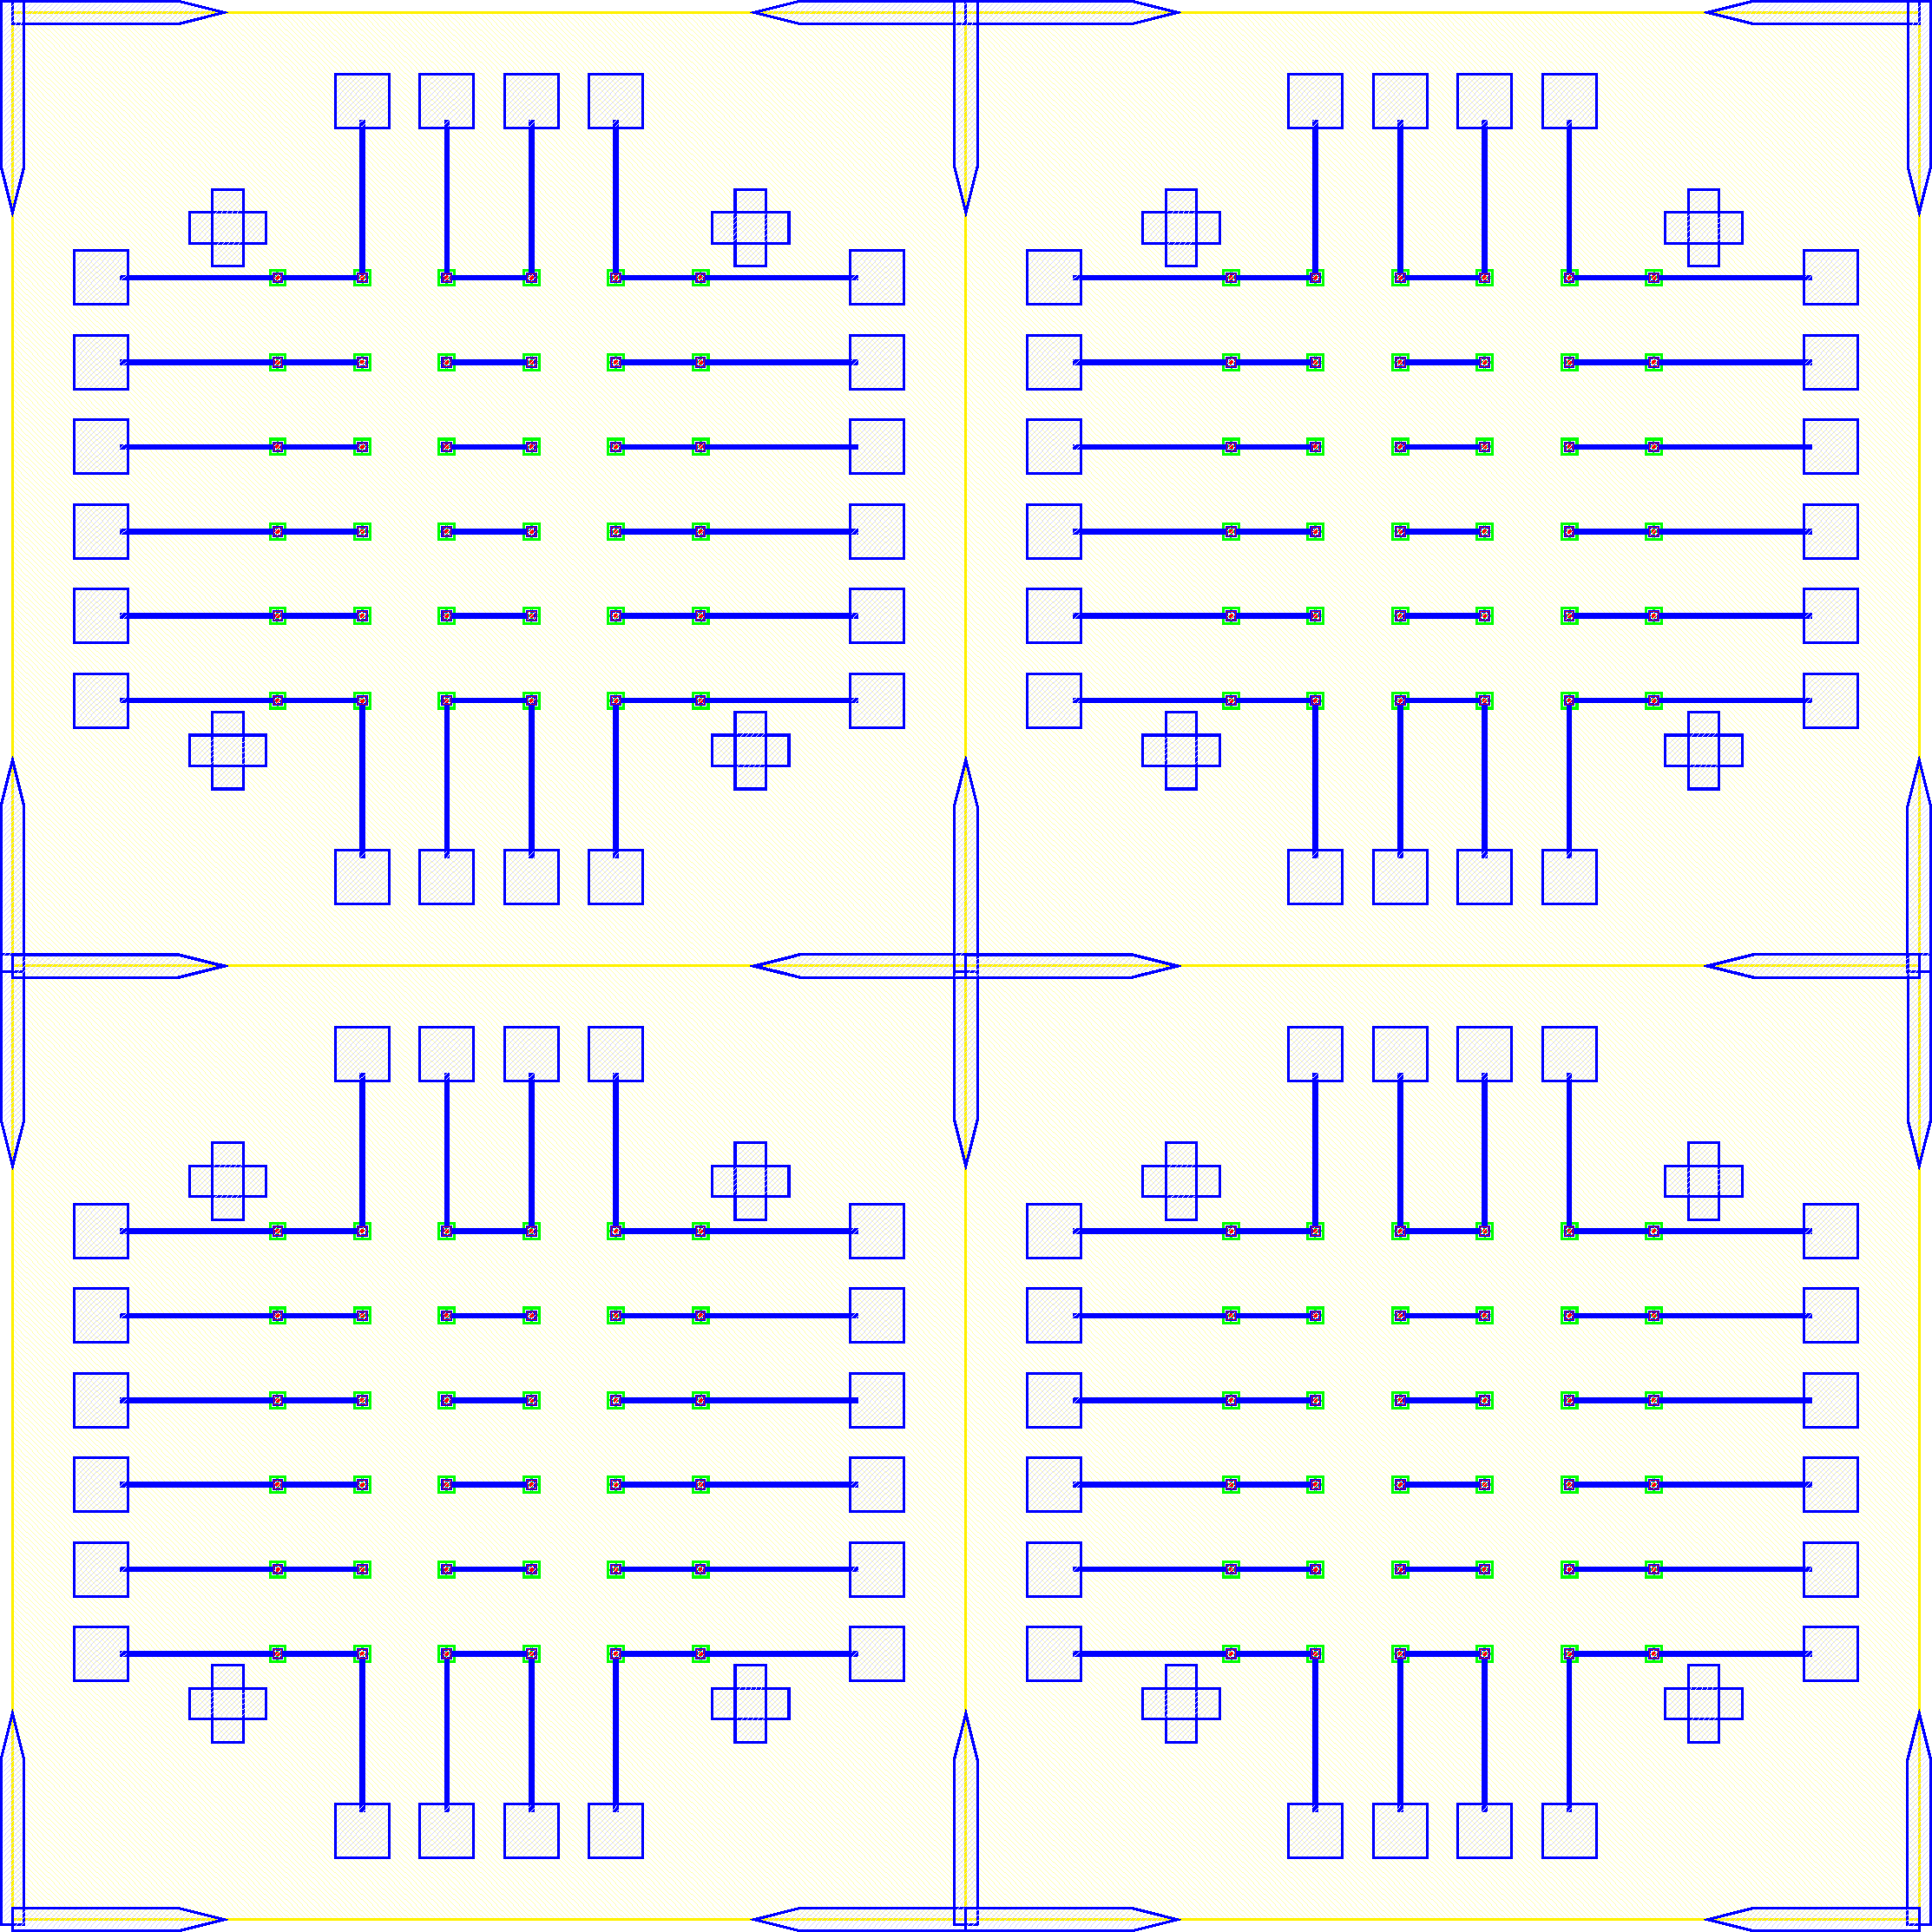
\includegraphics[width=0.6\textwidth]{Main/Ch2/DC_DieBTest_V2.GDStex_output.pdf}
    \caption{GDS file of electroplating sample. Green indicates the locations with indium electroplated. }
\end{figure}


% Specify [NUM] for wrapping # of lines b/w wrapfig and L
\begin{figure}
    \centering
    \begin{tikzpicture}
        \def\Ar{1.5 } % Radius
        \def\Ah{2   } % Cylinder Height
        \def\Ay{0.5 } % Ellipse second radius

        \def\Br{3   } % Radius
        \def\Bd{6   } % Diameter
        \def\Bh{1   } % Cylinder Height
        \def\By{0.5 } % Ellipse second radius

        \def\Dx{2   } % Offset distance
        \def\Ty{-1.5} % text vertical offset distance
        % First cylinder
        \draw           (   0,     0) ellipse [x radius=\Ar, y radius=\Ay]; % top
        \draw[dashed]   ( \Ar,  -\Ah) arc     (  0:180:\Ar and \Ay); % base
        \draw           (-\Ar,  -\Ah) arc     (180:360:\Ar and \Ay); % base
        \draw           (-\Ar,  -\Ah) --      (-\Ar, 0);
        \draw           ( \Ar,  -\Ah) --      ( \Ar, 0);

        % Second cylinder
        \draw           (\Ar+\Br+\Dx,  -\Ah-\Ay+\By+\Bh) ellipse [x radius=\Br, y radius=\By]; % top
        \draw[dashed]   (\Ar+\Bd+\Dx,  -\Ah-\Ay+\By)     arc     (  0:180:\Br and \By); % base
        \draw           (\Ar+\Dx    ,  -\Ah-\Ay+\By)     arc     (180:360:\Br and \By); % base
        \draw           (\Ar+\Dx    ,  -\Ah-\Ay+\By+\Bh) --      (\Ar+\Dx    , -\Ah-\Ay+\By);
        \draw           (\Ar+\Bd+\Dx,  -\Ah-\Ay+\By+\Bh) --      (\Ar+\Bd+\Dx, -\Ah-\Ay+\By);

        % Labels
        \node at        (          0, -1) {Electroplated bump};
        \node at        (\Ar+\Dx+\Br, -1) {Diebonded Bond};

        \draw [->,thick] (   \Ar*1.2, \Ty) ->       (\Ar+\Dx*0.9, \Ty);
        \path[draw, -latex', <->](\Ar+\Dx+\Bd+0.2, -\Ah-\Ay+\By+\Bh) -- node [text width=2.5cm,midway,below,align=center,rotate=90] { $0.65 \um$} (\Ar+\Dx+\Bd+0.2,  -\Ah-\Ay+\By);
        \path[draw, -latex', <->](-\Ar-0.2, 0) -- node [text width=3.5cm,midway,above,align=center,rotate=90] { Plating Thickness \\ $3-8 \um$} (-\Ar-0.2,  -\Ah);
        \end{tikzpicture}
    \caption{Line drawing of the change in shape of indium shape (not to scale).}
\end{figure}


Based on a number of bonding experiments I determined that the average thickness of indium after bonding was around $0.65 \um$ a sample of the indium bump can be seen in figure \ref{fig:semIndium}

\begin{figure}
    \centering
    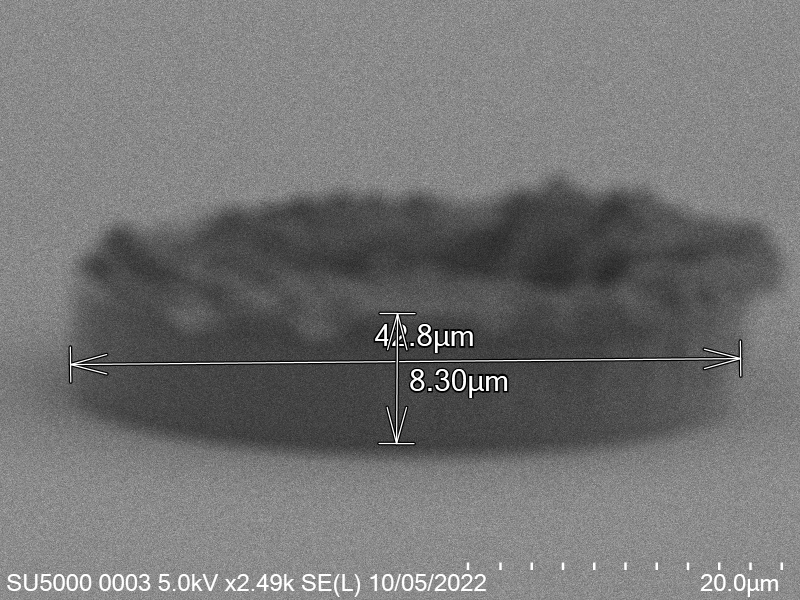
\includegraphics[width=0.45\textwidth]{Main/Ch2/indium_bump_before_bond.png}
    \caption{SEM image of indium bump at an angle of $80^\circ$}
    \label{fig:semIndium}
\end{figure}

The raw data from which the average indium thickness is determined table \ref{tab:thicknessMap}.

\begin{table}
    \centering
    \renewcommand{\minval}{0.1}
    \renewcommand{\maxval}{3}
    \begin{tabular}{| l | p{2.1cm} | p{2.3cm} | p{1.9cm} | p{1.9cm} | p{2.4cm}|}
    \hline
    Bond ID  &  $\ch{In}$ Bond Avg. Diameter ($\um$)  &  $\ch{In}$ Bump Thickness ($\um$)  &  $\ch{In}$ Bump Width ($\um$)  &  $\ch{In}$ Bump Volume ($\um^3$)  &  Bond Estimated Thickness ($\um$)
    \\
    \hline
    \hline
    BID-005  &  58.6  & 1.3   & 42 & 1801   & \grd{0.667} \\
    BID-006  &  84    & 1.7   & 42 & 2355   & \grd{0.425} \\
    BID-008  &  200   & 14    & 42 & 19396  & \grd{0.617} \\
    BID-009  &  86    & 8.4   & 42 & 11637  & \grd{2.003} \\
    BID-010  &  105   & 8.3   & 42 & 11499  & \grd{1.328} \\
    BID-011  &  142   & 8.5   & 42 & 11776  & \grd{0.743} \\
    BID-012  &  164   & 10    & 42 & 13854  & \grd{0.655} \\
    \hline
    \hline
    \end{tabular}
    \caption{Table of estimated thickness post diebonding}
    \label{tab:thicknessMap}
\end{table}

From the table after removing outlier values, the median resulting thickness is $ ~65 \um $.

The spread values were identified from images taken from the microscope `OLYMPUS-scope3' in the packaging lab.

From the images captured by the scope \ref{fig:microscopeIndium}, we can see that the gimbal head in the lab provides sufficiently uniform bonding pressure over the bonding area. The images also show that there is spreading of the indium as the bond is formed directly as a function of the indium volume. This is clear from the fact that the initial electroplated area indicated in a light grey is $42\um$ in size and the spread area indicated in dark grey is around $100 \um$ in size.

This corresponds to what we see in \ref{eq:radius_indium}. Where the initial height of the indium growth from what we expect in \ref{fig:scatterplot} where the growth is estimated to be $4-5\um$ in thickness.


\begin{equation} \label{eq:radius_indium2}
    \begin{split}
        \sqrt{\frac{h_{Initial}}{ 0.65 \um}} 21 \um &= r_{Final} \um \\
        52.1 &\approx 50 \um
    \end{split}
\end{equation}


Knowing that the bond does spread will constrain the maximum density of \uleds \ for a given bump thickness.

\begin{figure}
    \centering
    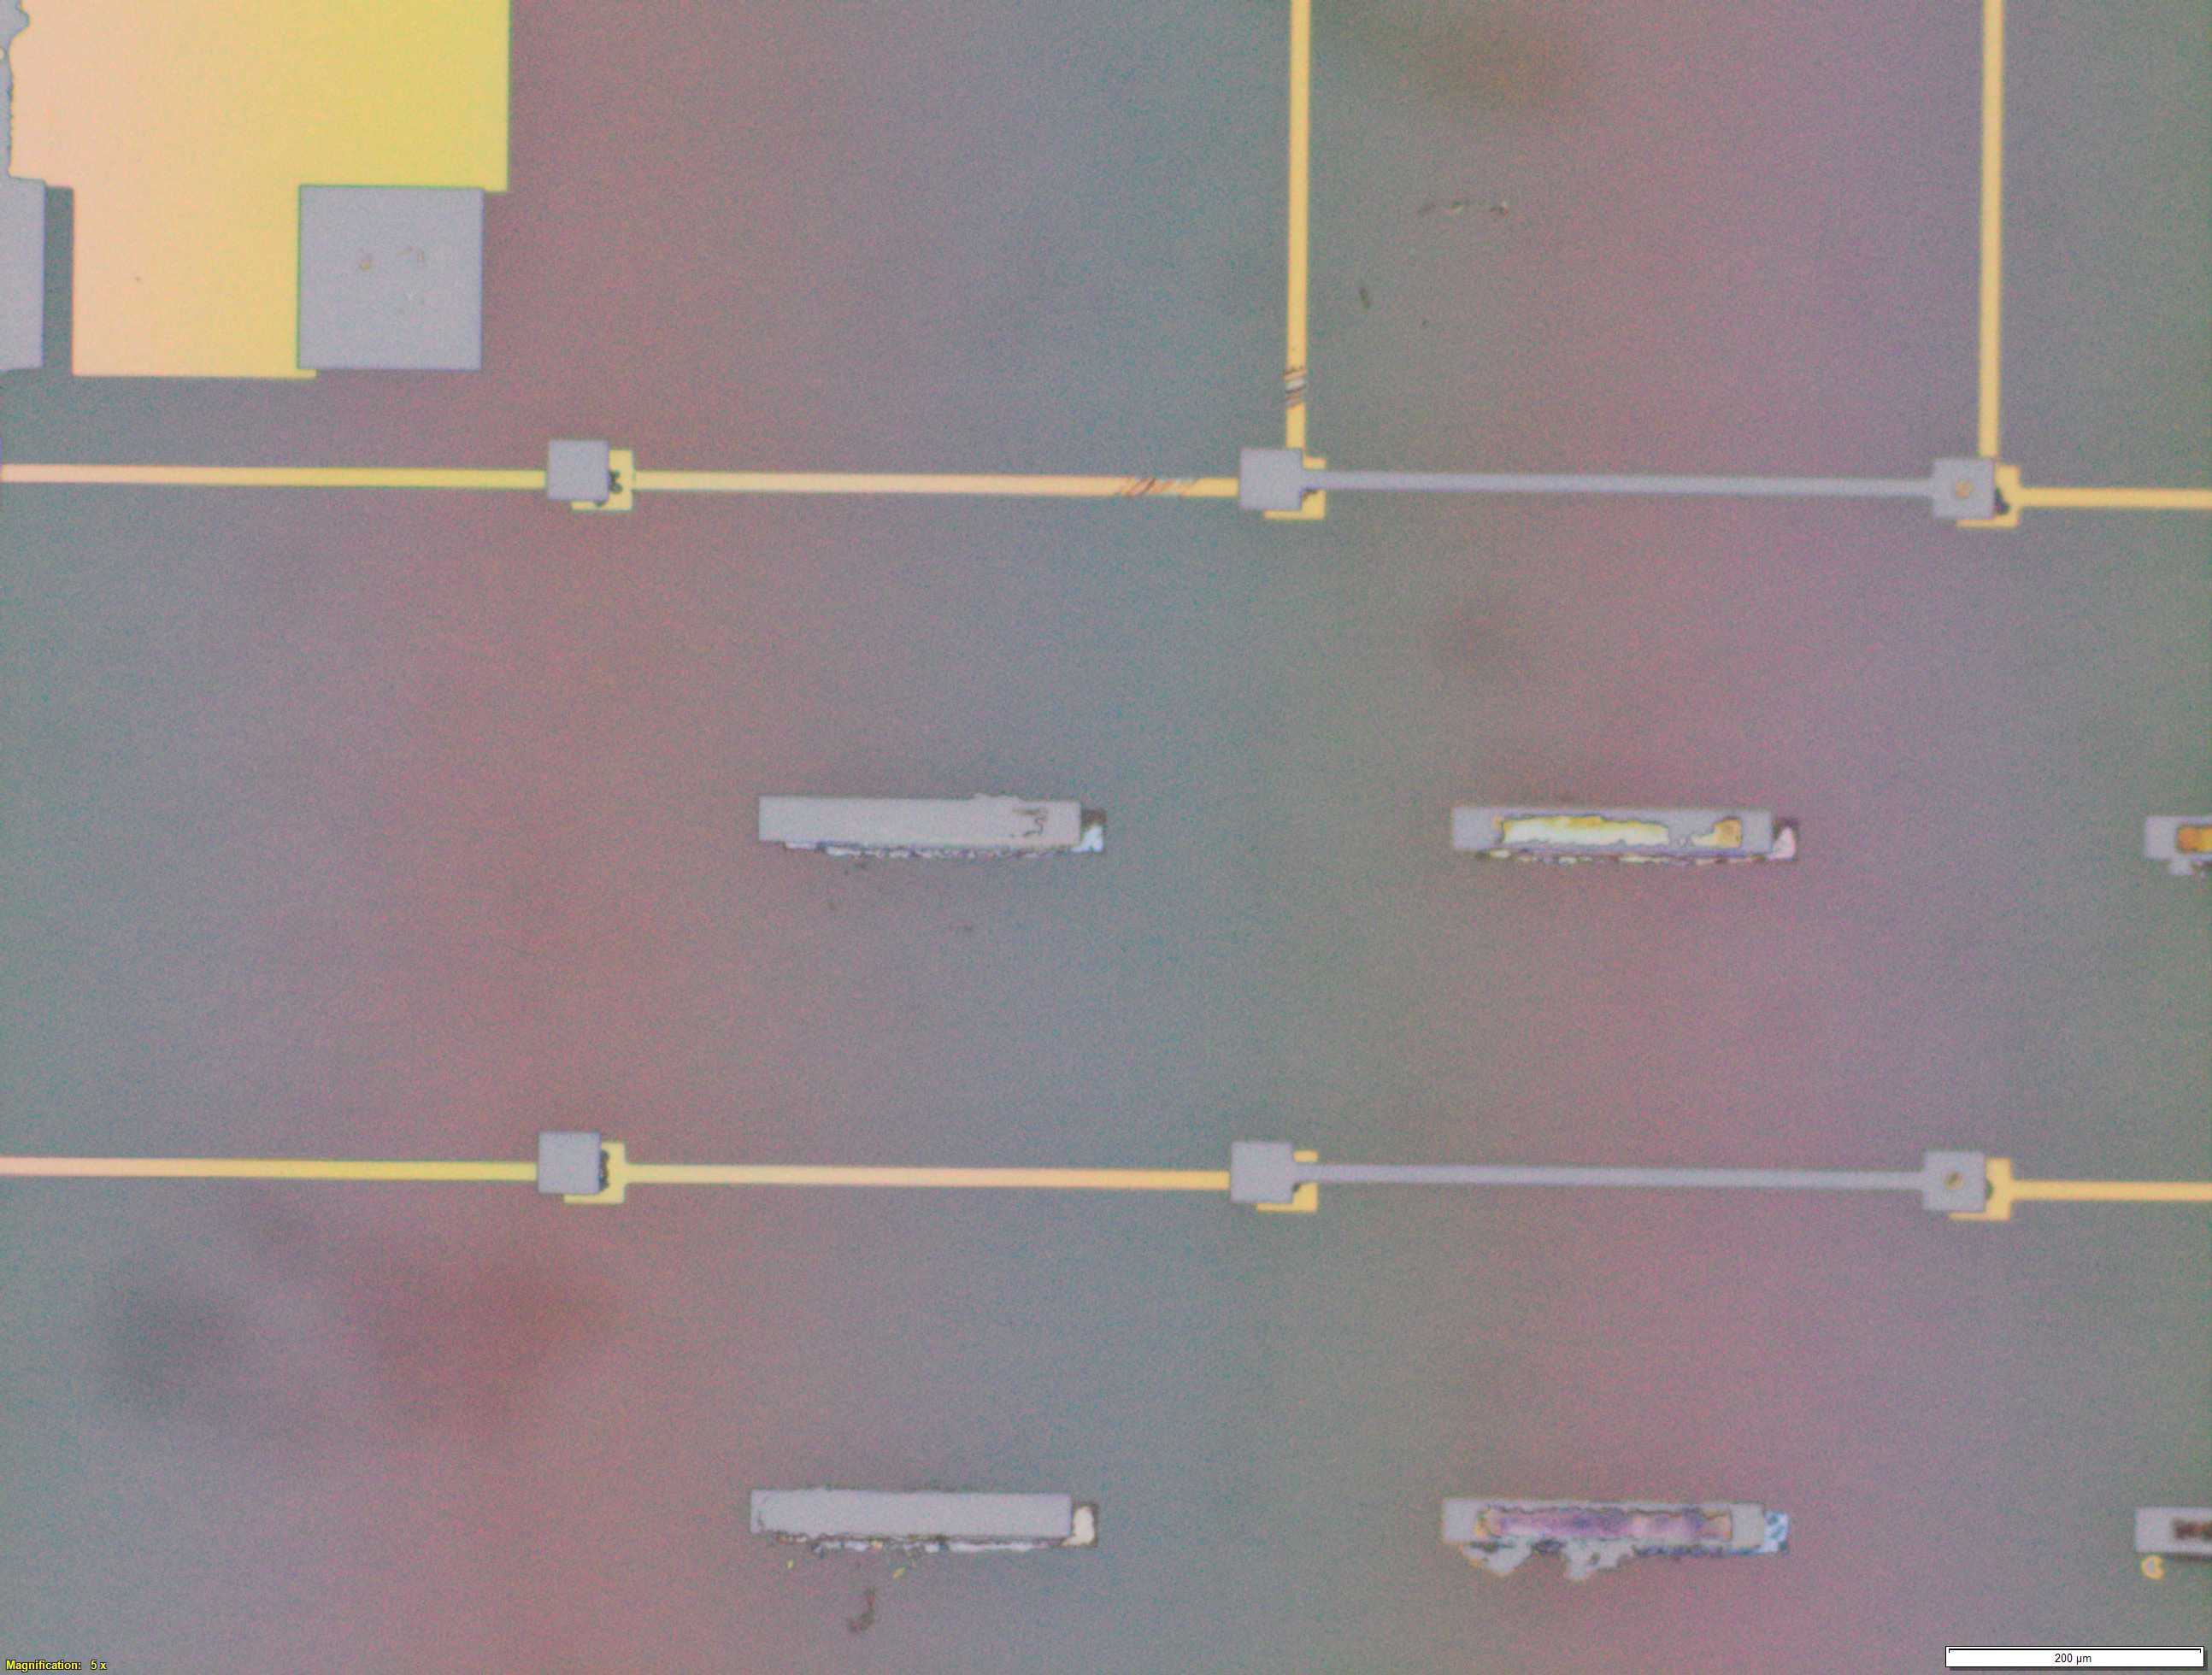
\includegraphics[width=0.22\textwidth]{Main/Ch2/microscopeGoodSpread/TL.png}
    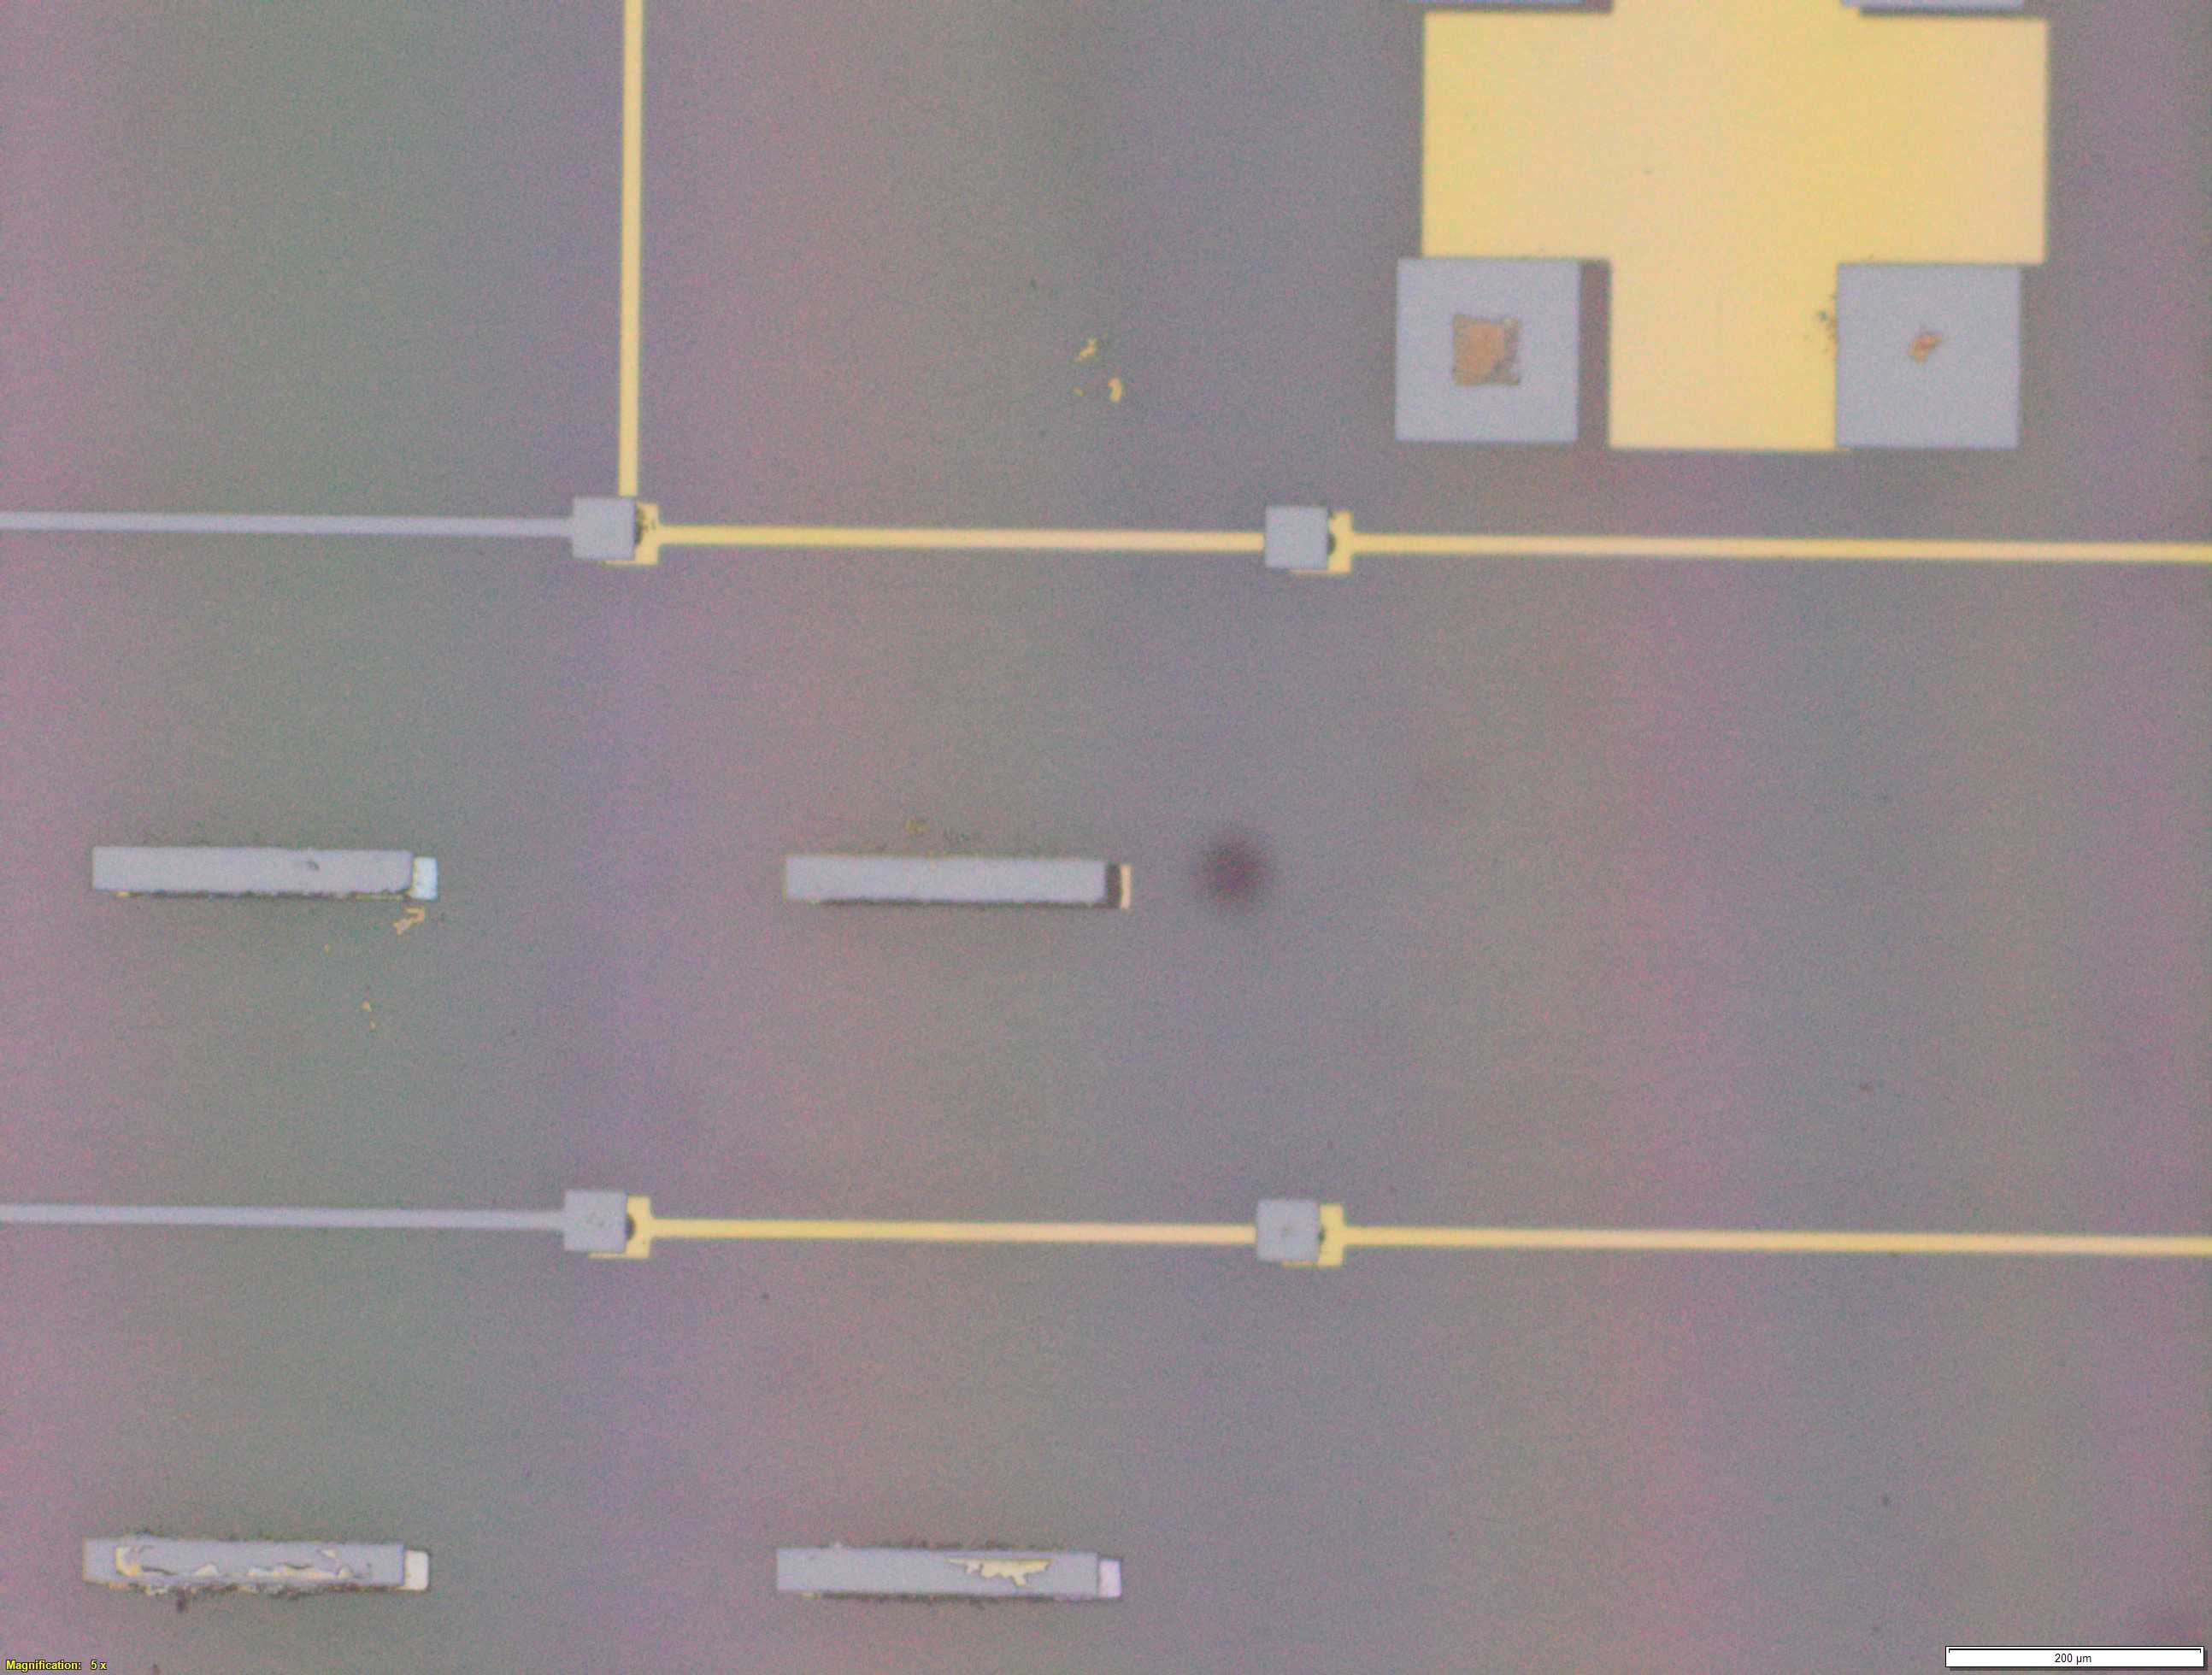
\includegraphics[width=0.22\textwidth]{Main/Ch2/microscopeGoodSpread/TR.png} \\
    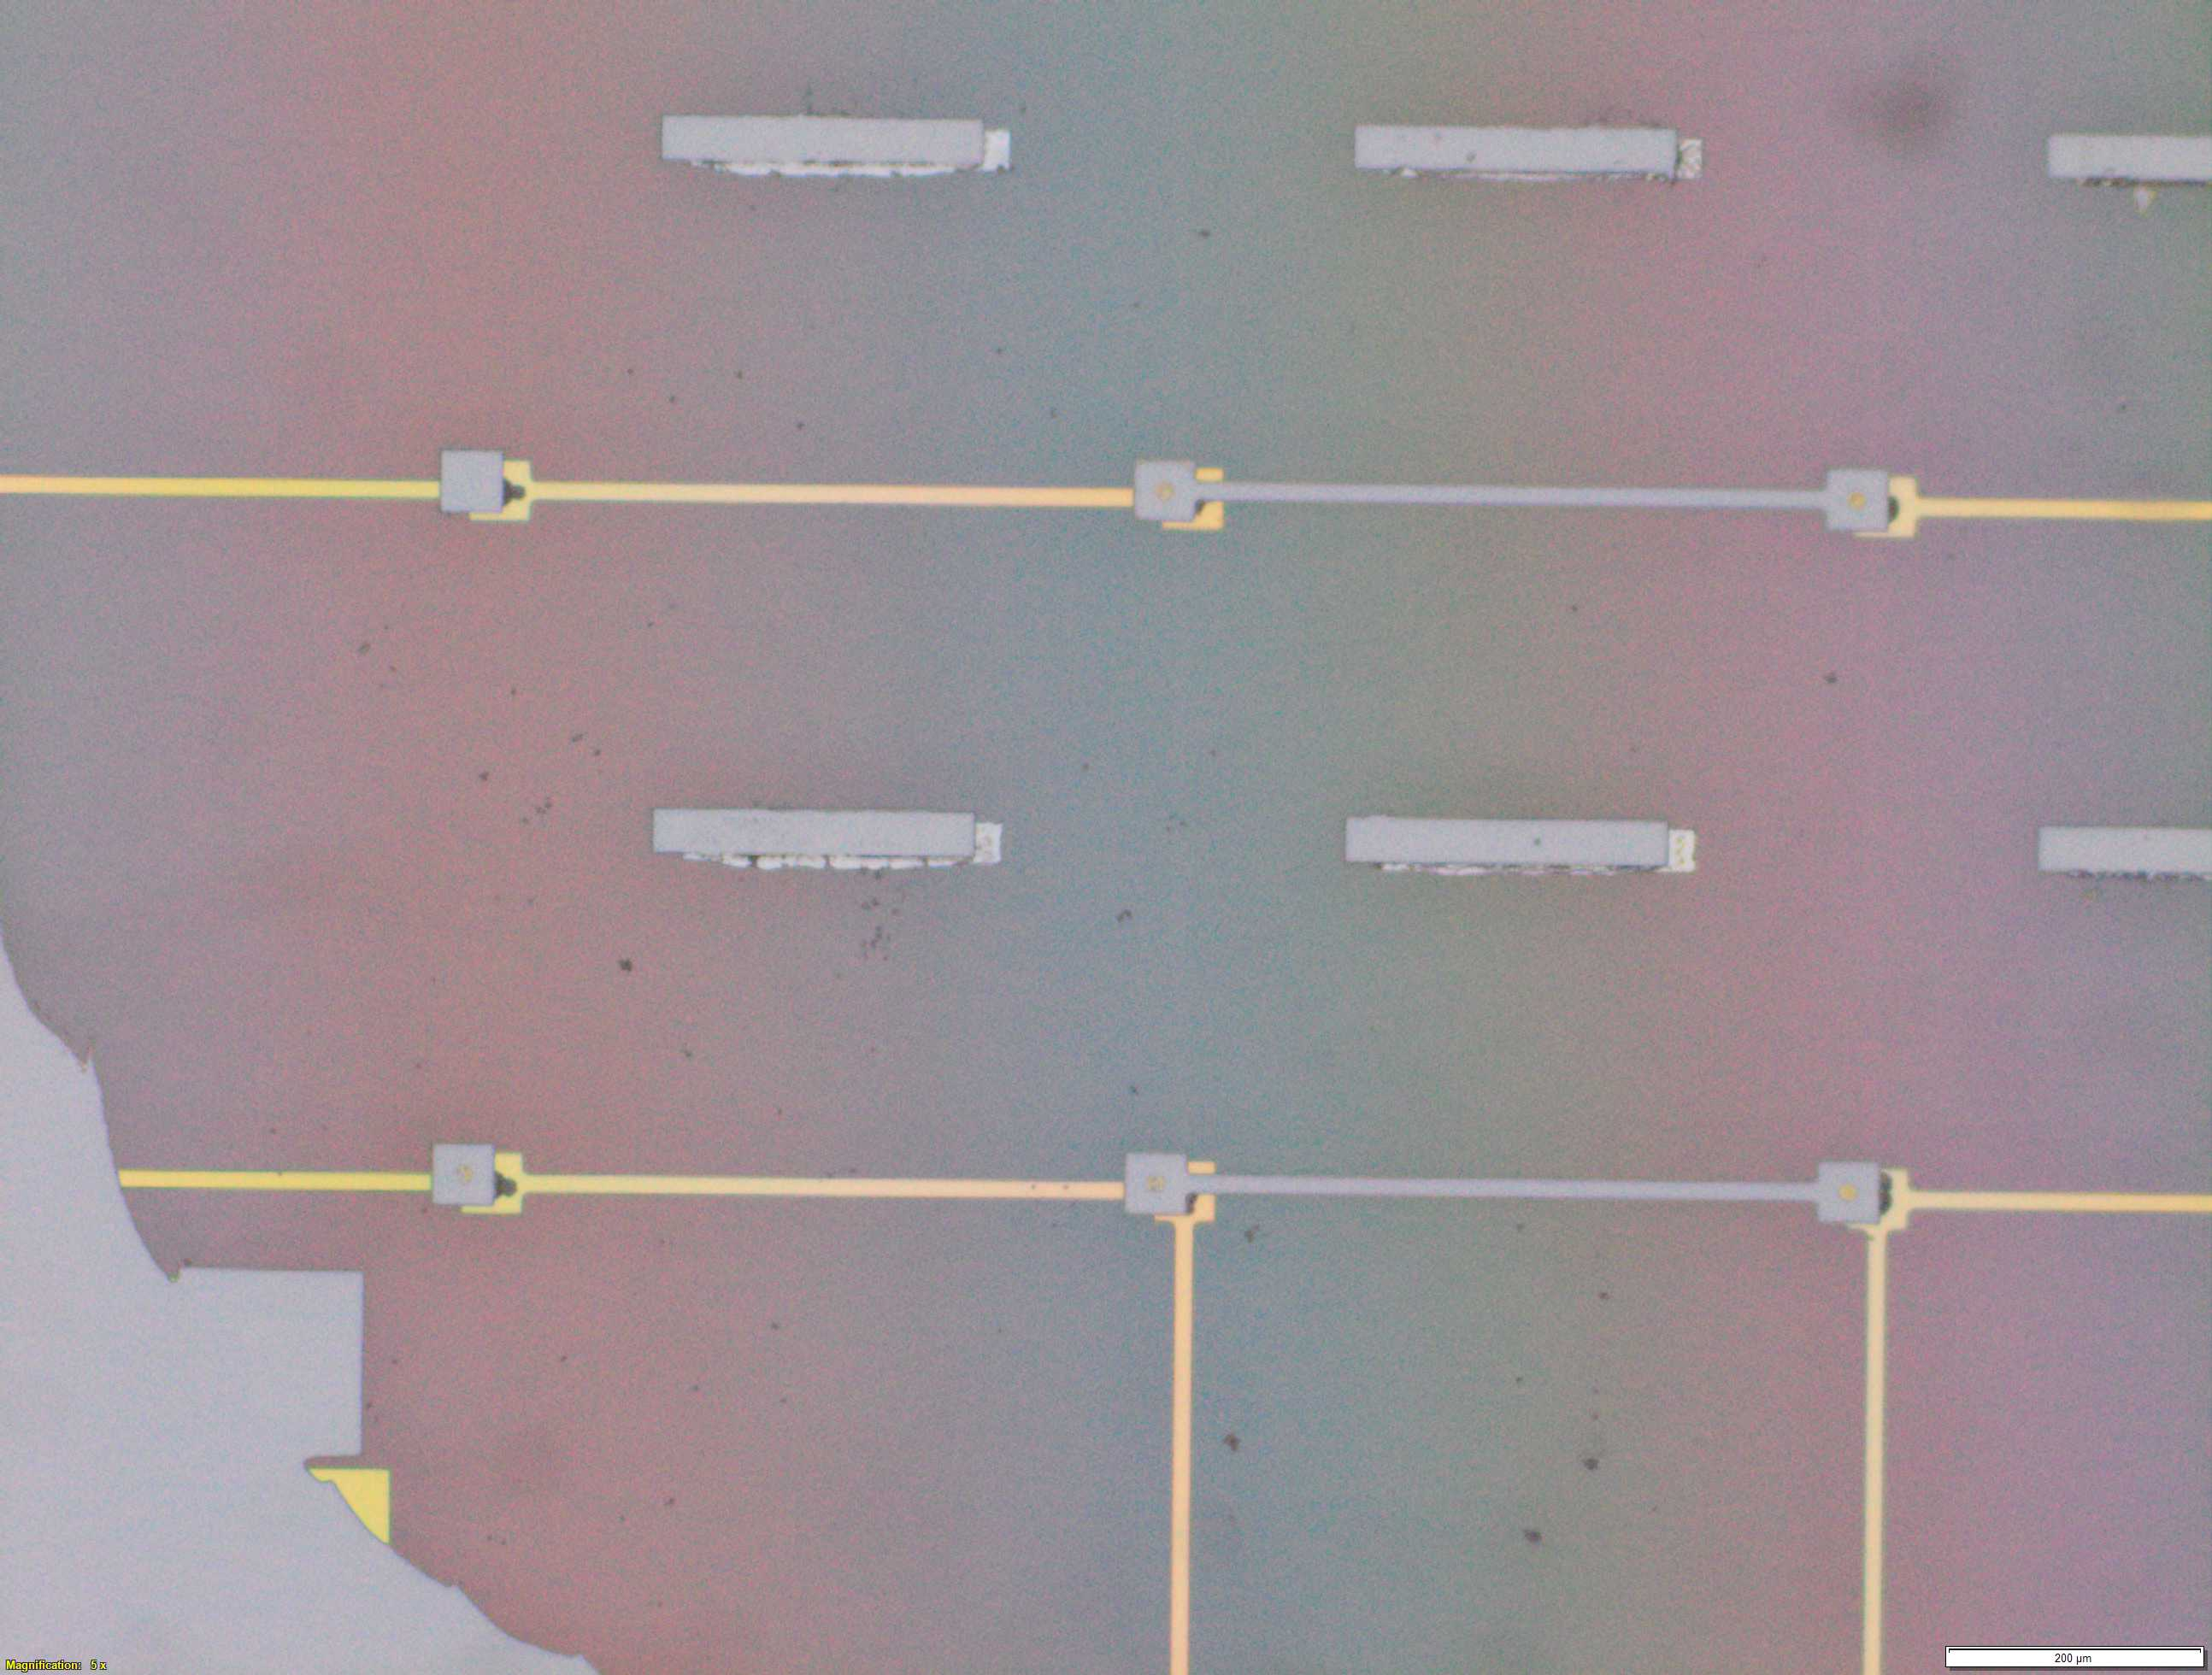
\includegraphics[width=0.22\textwidth]{Main/Ch2/microscopeGoodSpread/BL.png}
    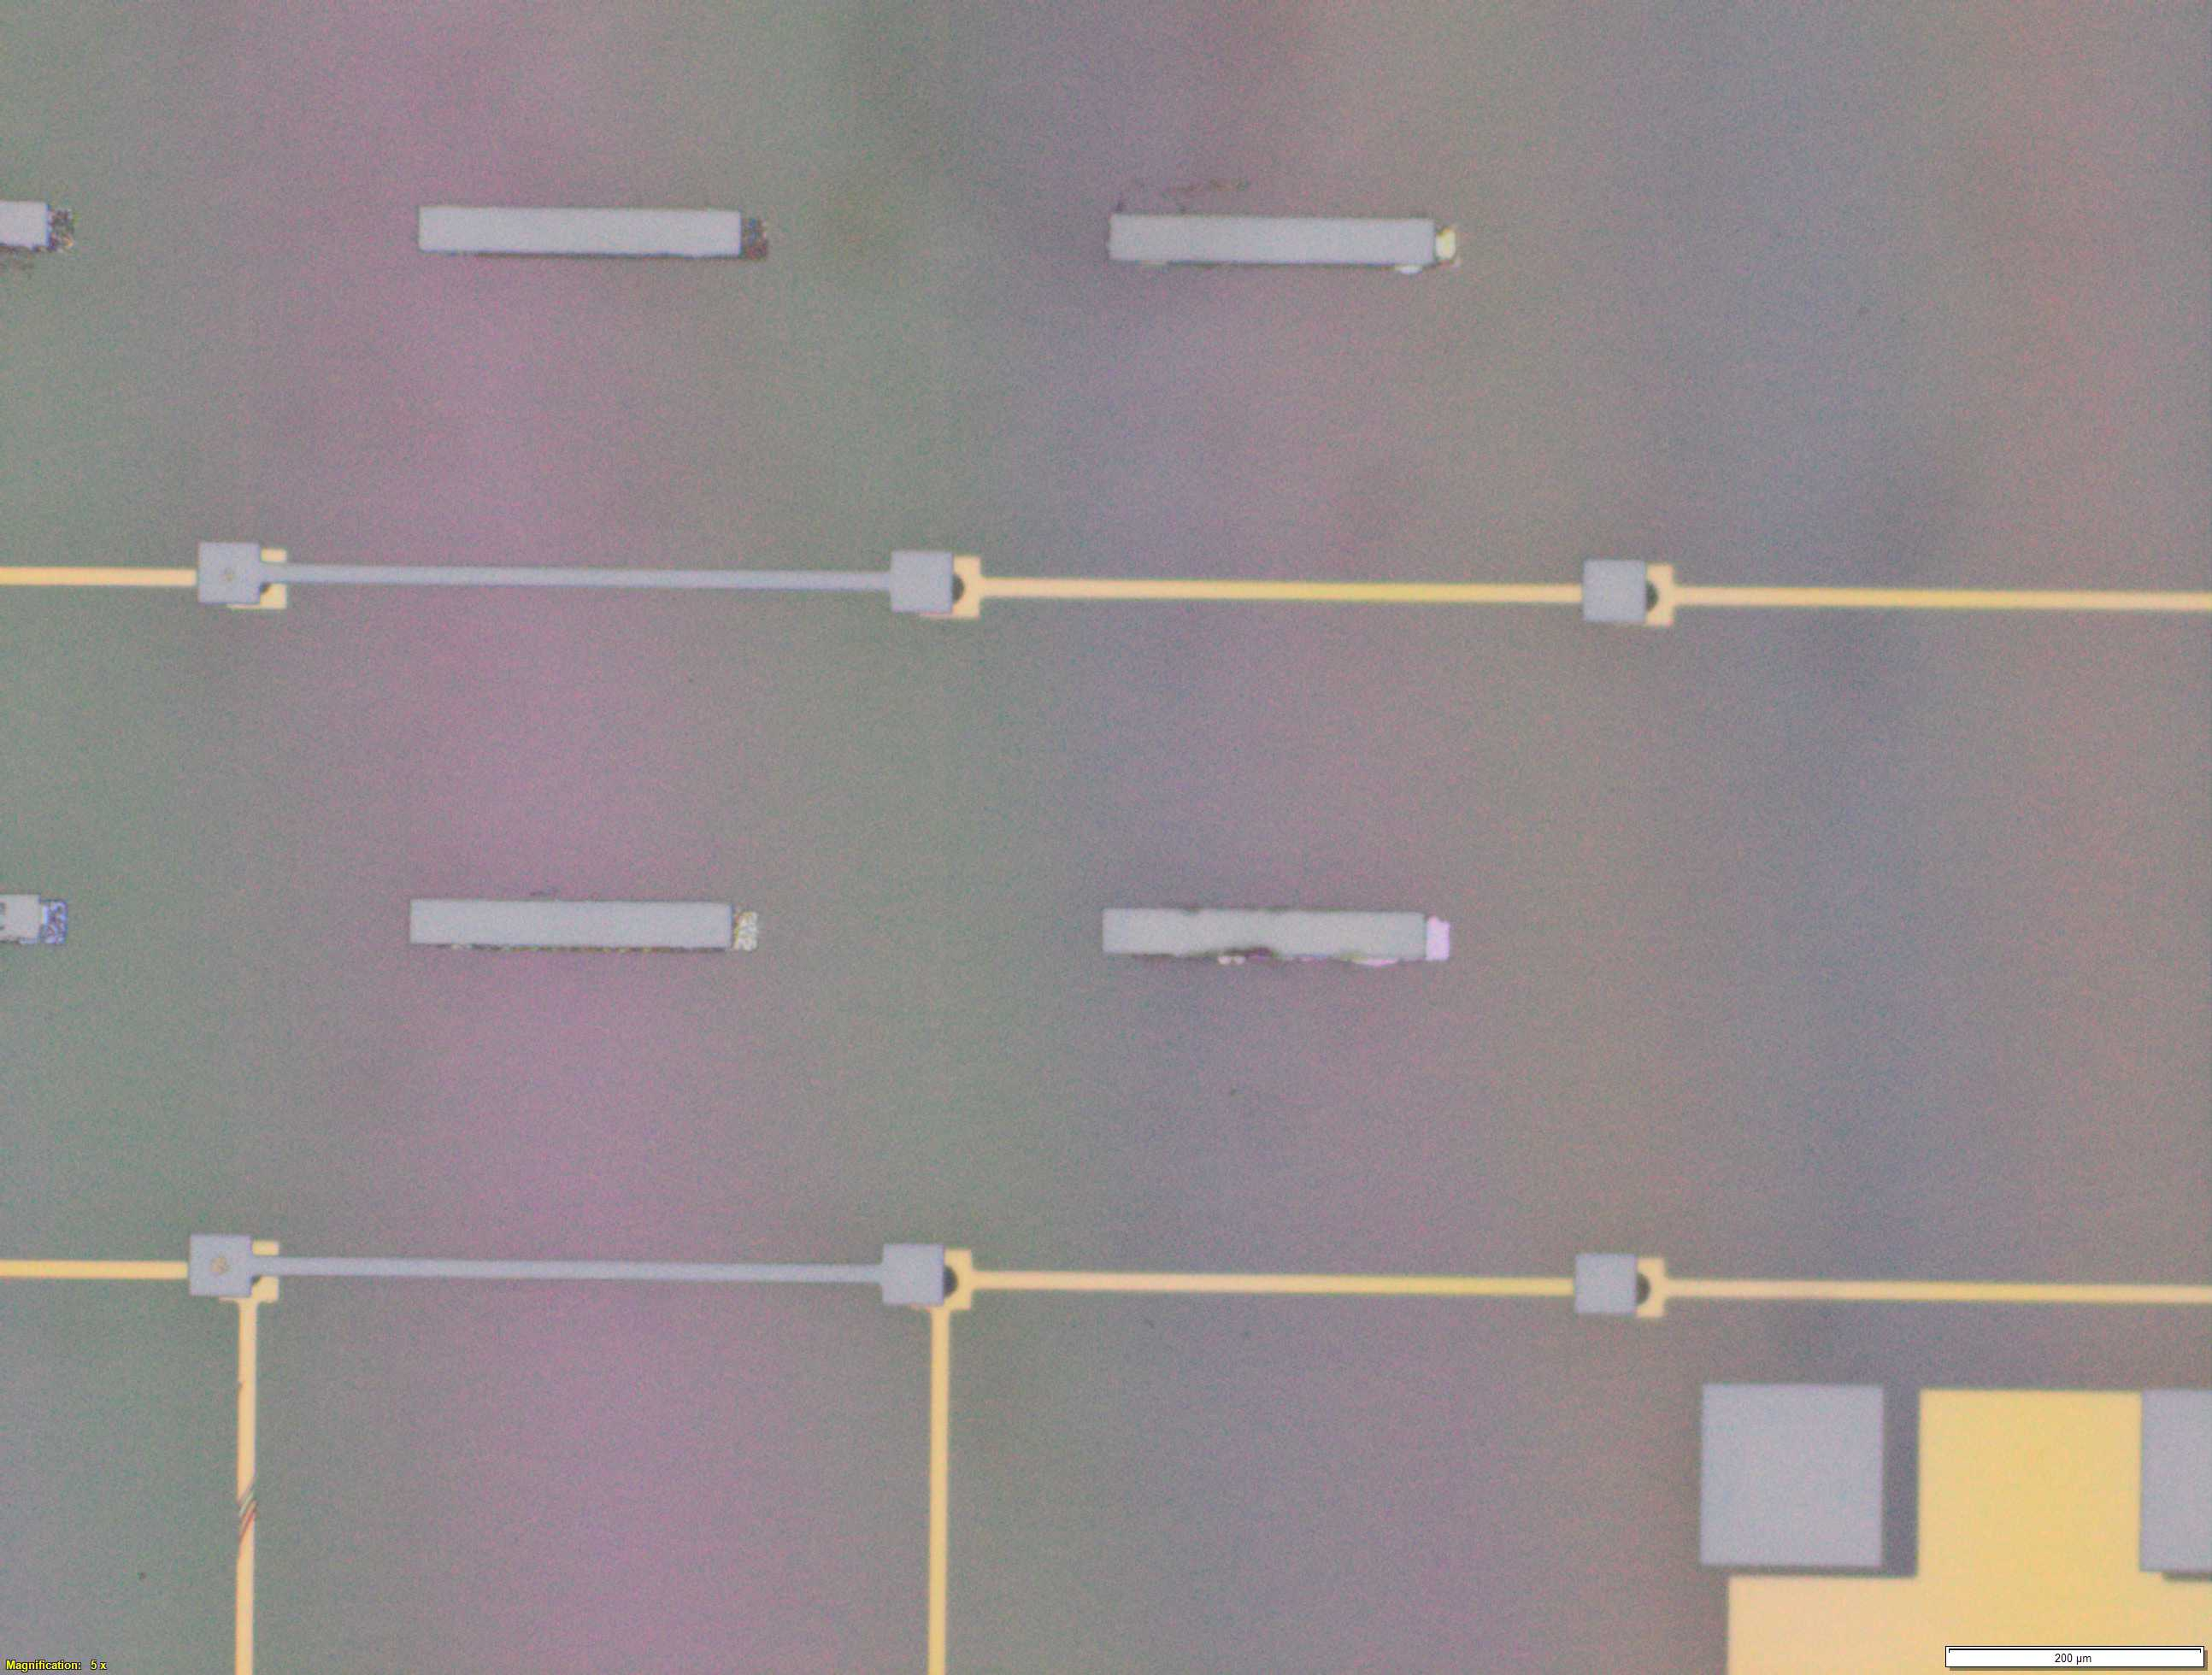
\includegraphics[width=0.22\textwidth]{Main/Ch2/microscopeGoodSpread/BR.png}
    \caption{Microscope images of diebonded sample. The internal smaller circles seen are a diameter of $42 \um$ the larger circles are the indium spreading}
    \label{fig:microscopeIndium}
    % \vspace{0.5cm}
\end{figure}

\section{Validation of Uniform Bonding}
\label{sec:uniformBond}
To validate that the bonding of the LEDs to the BP was uniform microscope images of the bonds were taken from the LED into the bond surface. As the LEDs for this phase of tests are largely transparent and mainly just dots of gold, it is very easy to see the spread of the indium bonds, this can be seen in the images in figure \ref{fig:microscopeIndium}

The gimbal head that is used has a structure like what is seen in figure \ref{fig:gimbal_head}
allows for

\begin{figure}
    \centering
    \begin{tikzpicture}
        \def\l{6cm}
        \def\t{12pt}

        \draw[draw=none, fill=CadetBlue!50]            (0, 0)          rectangle (\l, \t)           node[midway, right, xshift=\l/4] {Steel};
        \draw[draw=none, fill=purple4!50]              (0, \t)         rectangle (\l, \t*2)         node[midway, right, xshift=\l/4] {Rubber};
        \draw[draw=none, fill=CadetBlue!50]            (0, \t*2)       rectangle (\l, \t*3)         node[midway, right, xshift=\l/4] {Steel};
        \draw[draw=none, fill=CadetBlue!50]            (\l*0.60, \t*2) rectangle (\l*0.40, \t*10);
        \draw[draw=none, fill=white, fill opacity=0.5] (\l*0.55, 0)    rectangle (\l*0.45, \t*10)   node[midway, rotate=90] {Vacuum hole};
    \end{tikzpicture}
    \caption{Gimbal head cross-section view (not to scale)}
    \label{fig:gimbal_head}
\end{figure}


% Reference to images of GDS files of the BP and LED

\section{Thermal Simulations}

Thermal simulations were conducted because there were some bonding failures seen in the samples. As can be seen from SEM images and Energy-dispersive X-ray spectroscopy (EDX or EDS) the indium does not always appropriately wet onto the other substrate being bonded onto this is seen in the SEM images in figure
\ref{fig:SEM_indium_2} and EDX images in figure \ref{fig:EDX_indium_2}.
There can be various reasons why indium does not wet onto a surface during diebonding. One reason could be the presence of surface contaminants such as oxides or oils, which can prevent the indium from bonding to the surface. Another reason could be an insufficient amount of heat or pressure during the diebonding process, which can cause the indium to not properly wet onto the surface. Additionally, the surface energy of the substrate can also affect the ability of indium to wet onto the surface during diebonding.

To explore further a lack of heat, thermal simulations were conducted to identify if a process change in the diebonding preprocess was required. Thermal simulations were done in MATLAB with the following code in
\hyperref[sec:ThermalSimulationCode]{Appendix B}.

\begin{figure}[h]
    \centering
\begin{subfigure}[t]{0.4\textwidth}
    \centering
    \begin{tabular}{c c c c}
    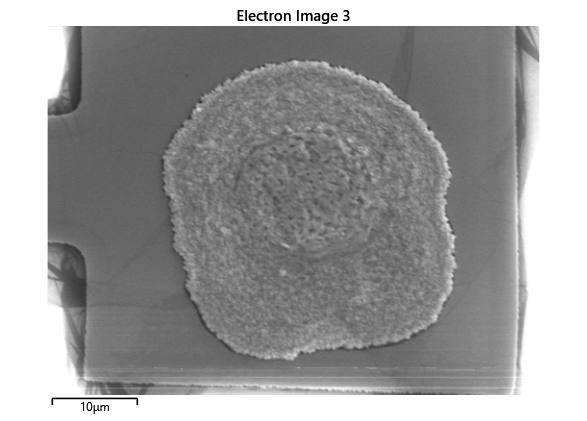
\includegraphics[height=1cm]{Main/Ch2/extracted/SEM/In-EP-EDx_TBP-01-A1-s1_media_image.png} &
    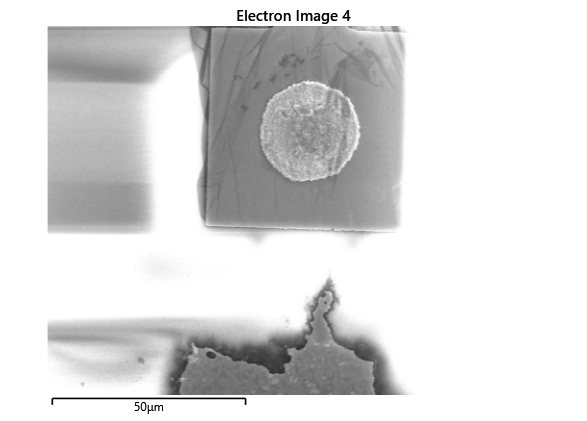
\includegraphics[height=1cm]{Main/Ch2/extracted/SEM/In-EP-EDx_TBP-01-A1-s2_media_image.png} &
    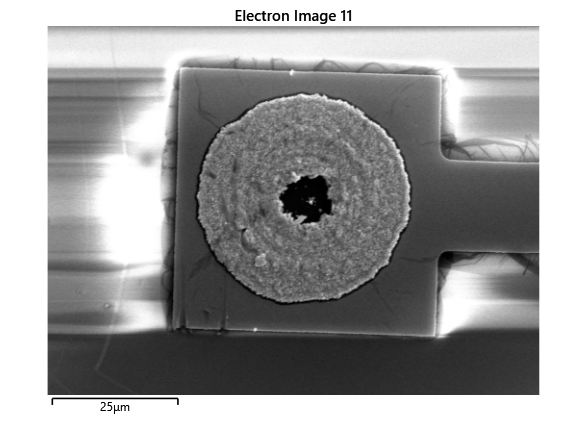
\includegraphics[height=1cm]{Main/Ch2/extracted/SEM/In-EP-EDx_TBP-01-A2-s1_media_image.png} &
    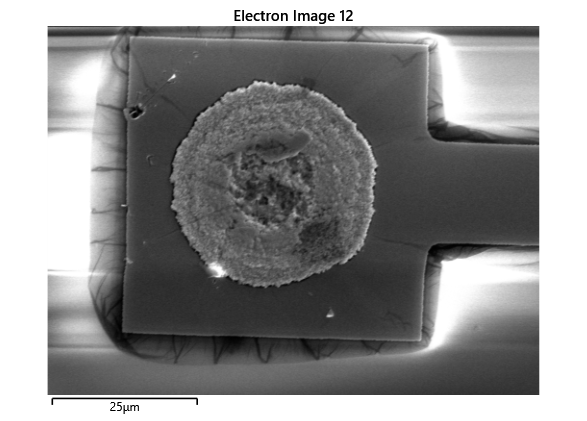
\includegraphics[height=1cm]{Main/Ch2/extracted/SEM/In-EP-EDx_TBP-01-A2-s2_media_image.png} \\
    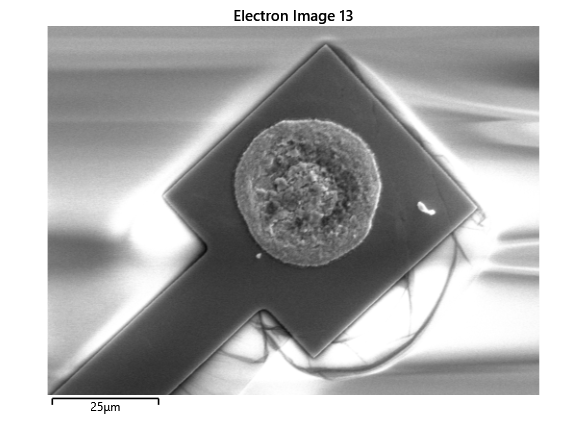
\includegraphics[height=1cm]{Main/Ch2/extracted/SEM/In-EP-EDx_TBP-01-B2-s1_media_image.png} &
    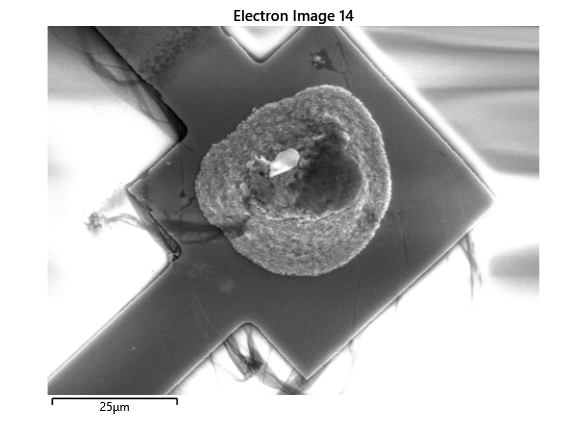
\includegraphics[height=1cm]{Main/Ch2/extracted/SEM/In-EP-EDx_TBP-01-B2-s2_media_image.png} &
    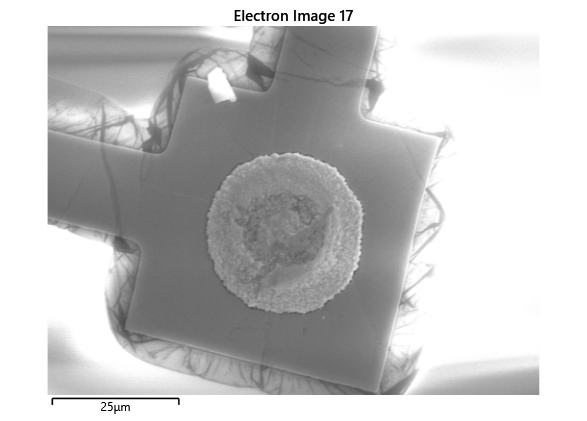
\includegraphics[height=1cm]{Main/Ch2/extracted/SEM/In-EP-EDx_TBP-02-A1-s1_media_image.png} &
    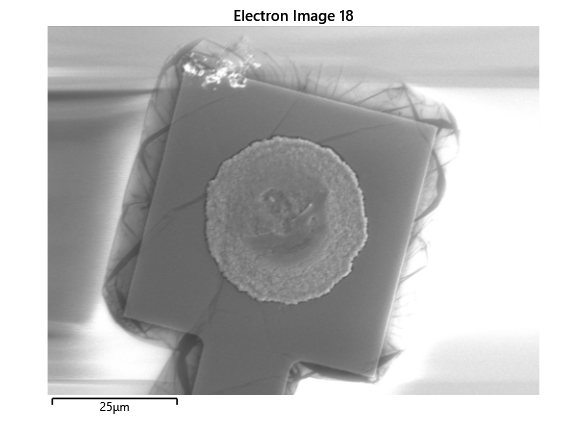
\includegraphics[height=1cm]{Main/Ch2/extracted/SEM/In-EP-EDx_TBP-02-A1-s2_media_image.png} \\
    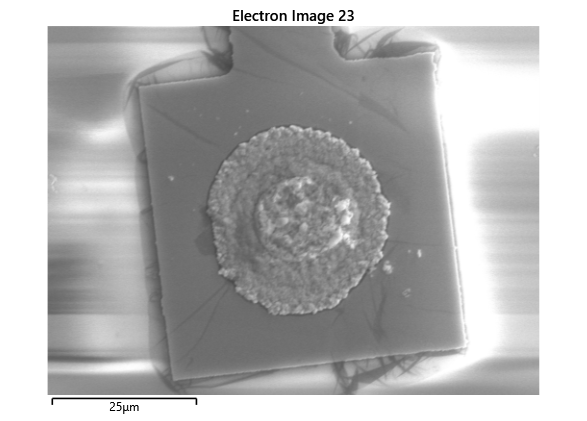
\includegraphics[height=1cm]{Main/Ch2/extracted/SEM/In-EP-EDx_TBP-02-A2-s1_media_image.png} &
    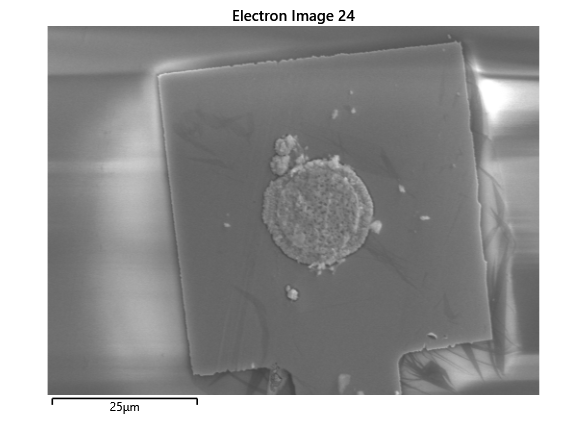
\includegraphics[height=1cm]{Main/Ch2/extracted/SEM/In-EP-EDx_TBP-02-A2-s2_media_image.png} &
    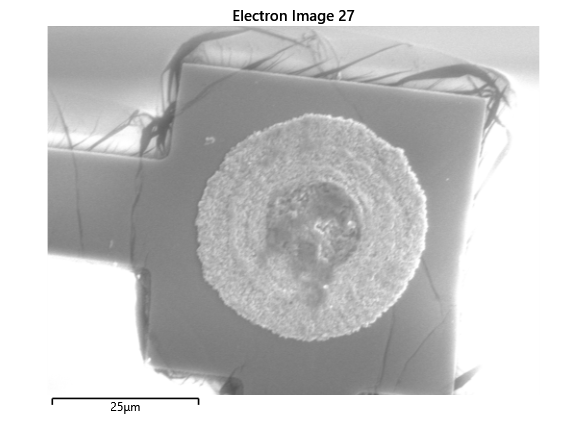
\includegraphics[height=1cm]{Main/Ch2/extracted/SEM/In-EP-EDx_TBP-02-B2-s1_media_image.png} &
    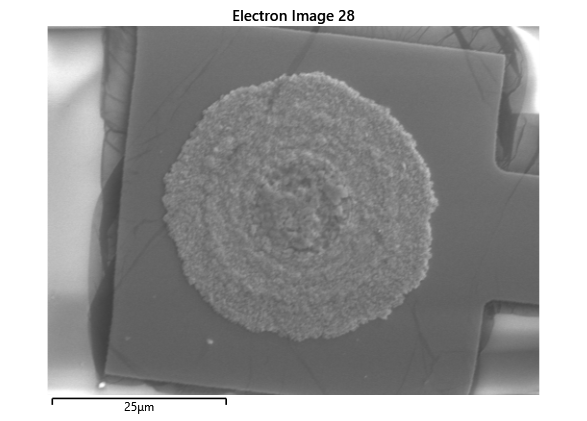
\includegraphics[height=1cm]{Main/Ch2/extracted/SEM/In-EP-EDx_TBP-02-B2-s2_media_image.png} \\
    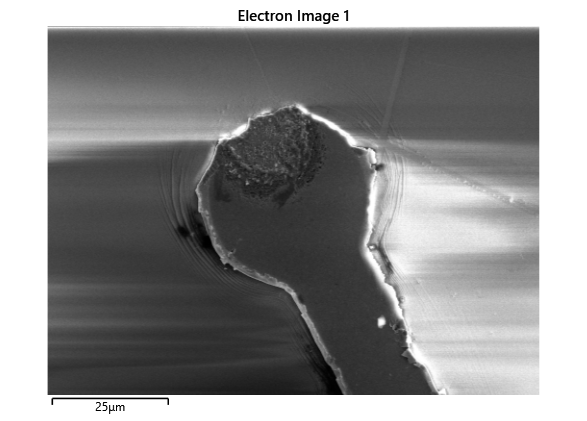
\includegraphics[height=1cm]{Main/Ch2/extracted/SEM/In-EP-EDx_TLED-01-A1-s1_media_image.png} &
    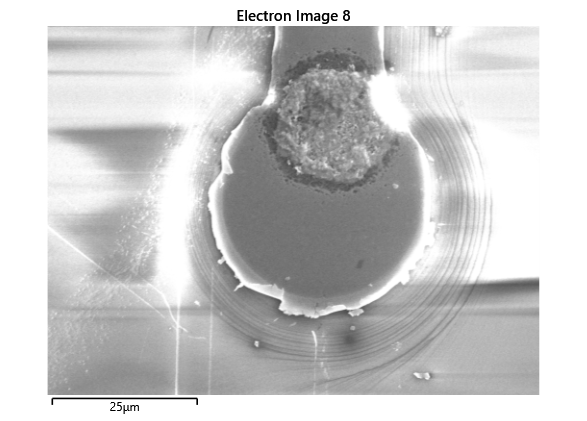
\includegraphics[height=1cm]{Main/Ch2/extracted/SEM/In-EP-EDx_TLED-01-A1-s2_media_image.png} &
    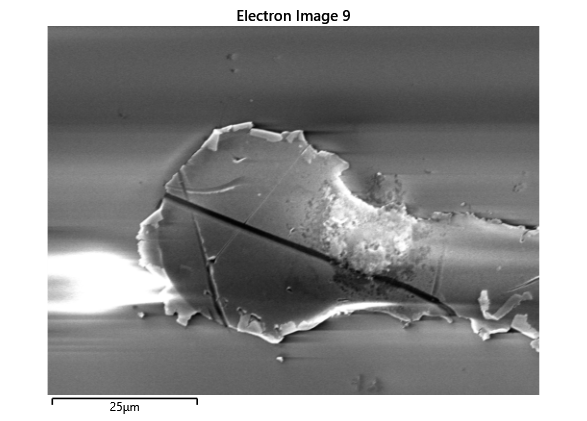
\includegraphics[height=1cm]{Main/Ch2/extracted/SEM/In-EP-EDx_TLED-01-A2-s1_media_image.png} &
    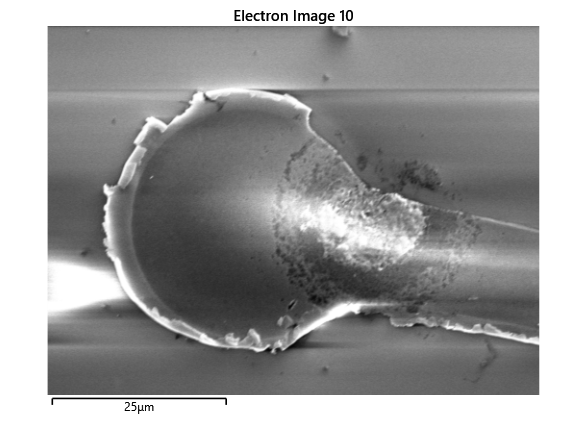
\includegraphics[height=1cm]{Main/Ch2/extracted/SEM/In-EP-EDx_TLED-01-A2-s2_media_image.png} \\
    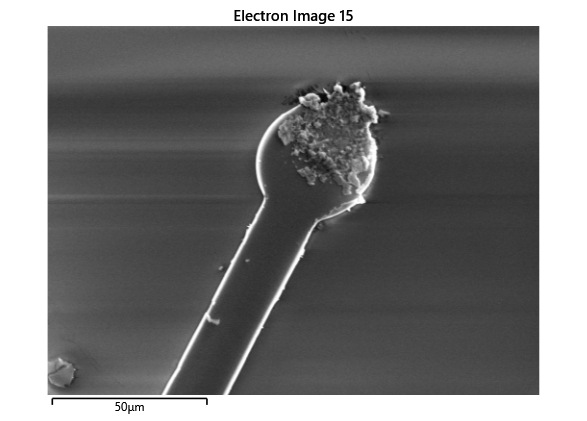
\includegraphics[height=1cm]{Main/Ch2/extracted/SEM/In-EP-EDx_TLED-01-B2-s1_media_image.png} &
    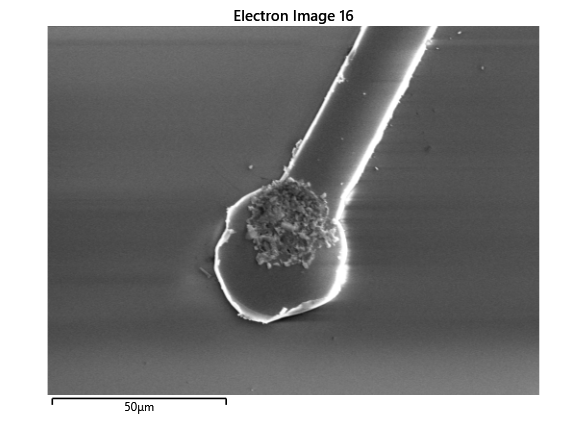
\includegraphics[height=1cm]{Main/Ch2/extracted/SEM/In-EP-EDx_TLED-01-B2-s2_media_image.png} &
    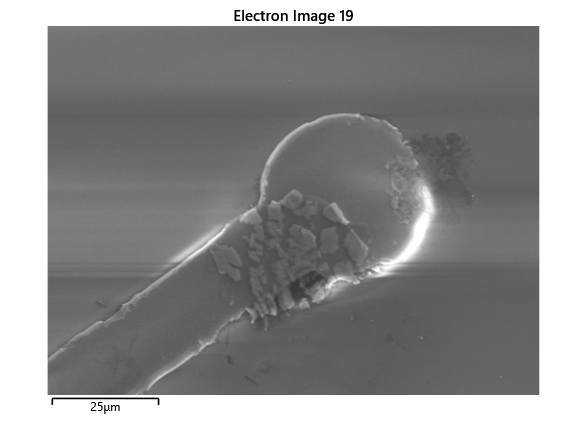
\includegraphics[height=1cm]{Main/Ch2/extracted/SEM/In-EP-EDx_TLED-02-A1-s1_media_image.png} &
    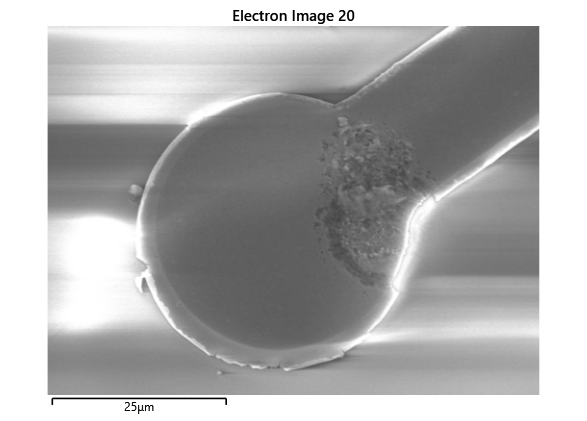
\includegraphics[height=1cm]{Main/Ch2/extracted/SEM/In-EP-EDx_TLED-02-A1-s2_media_image.png} \\
    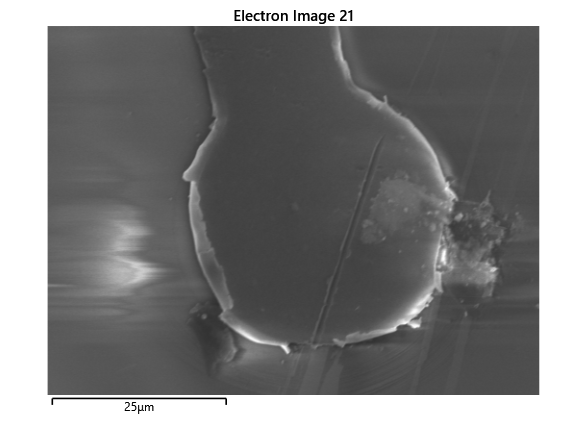
\includegraphics[height=1cm]{Main/Ch2/extracted/SEM/In-EP-EDx_TLED-02-A2-s1_media_image.png} &
    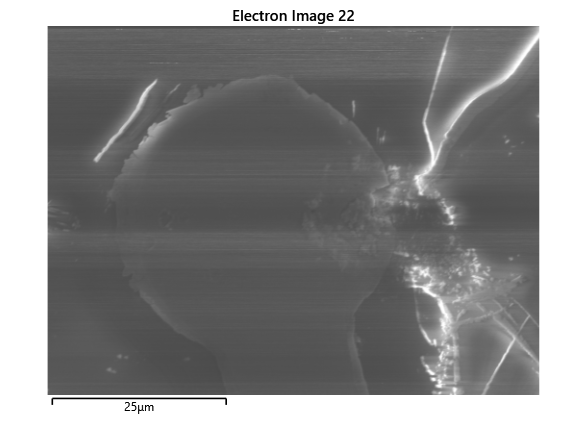
\includegraphics[height=1cm]{Main/Ch2/extracted/SEM/In-EP-EDx_TLED-02-A2-s2_media_image.png} &
    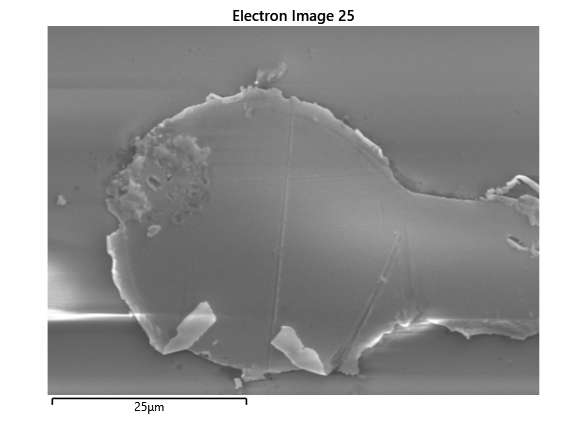
\includegraphics[height=1cm]{Main/Ch2/extracted/SEM/In-EP-EDx_TLED-02-B2-s1_media_image.png} &
    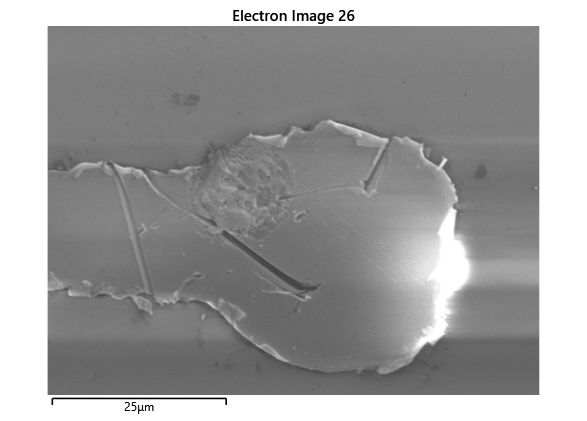
\includegraphics[height=1cm]{Main/Ch2/extracted/SEM/In-EP-EDx_TLED-02-B2-s2_media_image.png} \\
    \end{tabular}
    \caption{SEM Images of bonds}
    \label{fig:SEM_indium_2}
\end{subfigure}
~
\begin{subfigure}[t]{0.4\textwidth}
    \centering
    \begin{tabular}{c c c c}
    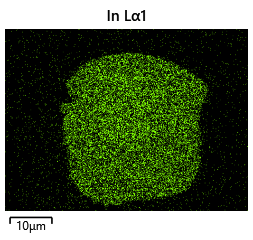
\includegraphics[height=1cm]{Main/Ch2/extracted/Indium/In-EP-EDx_TBP-01-A1-s1_media_image7.png} &
    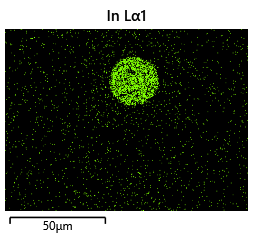
\includegraphics[height=1cm]{Main/Ch2/extracted/Indium/In-EP-EDx_TBP-01-A1-s2_media_image7.png} &
    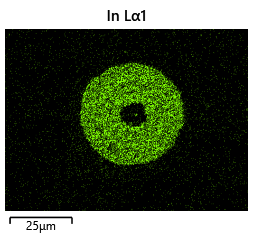
\includegraphics[height=1cm]{Main/Ch2/extracted/Indium/In-EP-EDx_TBP-01-A2-s1_media_image7.png} &
    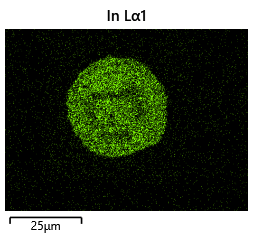
\includegraphics[height=1cm]{Main/Ch2/extracted/Indium/In-EP-EDx_TBP-01-A2-s2_media_image7.png} \\
    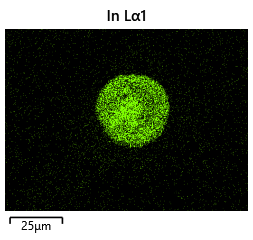
\includegraphics[height=1cm]{Main/Ch2/extracted/Indium/In-EP-EDx_TBP-01-B2-s1_media_image7.png} &
    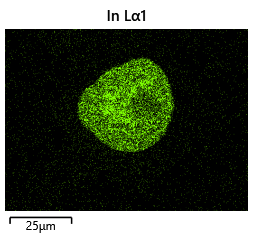
\includegraphics[height=1cm]{Main/Ch2/extracted/Indium/In-EP-EDx_TBP-01-B2-s2_media_image7.png} &
    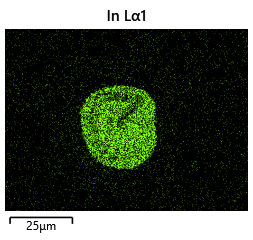
\includegraphics[height=1cm]{Main/Ch2/extracted/Indium/In-EP-EDx_TBP-02-A1-s1_media_image7.png} &
    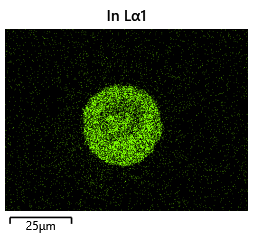
\includegraphics[height=1cm]{Main/Ch2/extracted/Indium/In-EP-EDx_TBP-02-A1-s2_media_image7.png} \\
    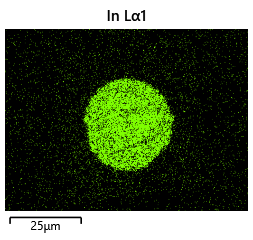
\includegraphics[height=1cm]{Main/Ch2/extracted/Indium/In-EP-EDx_TBP-02-A2-s1_media_image7.png} &
    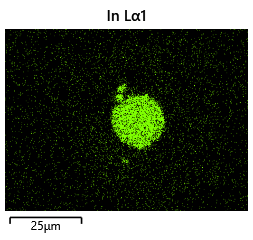
\includegraphics[height=1cm]{Main/Ch2/extracted/Indium/In-EP-EDx_TBP-02-A2-s2_media_image7.png} &
    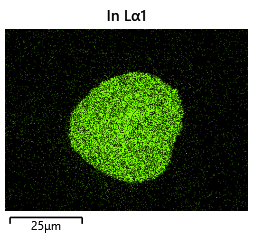
\includegraphics[height=1cm]{Main/Ch2/extracted/Indium/In-EP-EDx_TBP-02-B2-s1_media_image7.png} &
    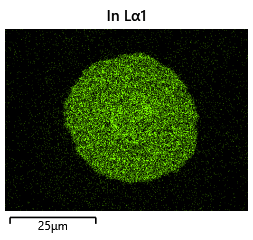
\includegraphics[height=1cm]{Main/Ch2/extracted/Indium/In-EP-EDx_TBP-02-B2-s2_media_image7.png} \\
    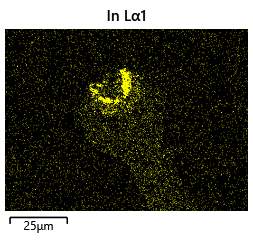
\includegraphics[height=1cm]{Main/Ch2/extracted/Indium/In-EP-EDx_TLED-01-A1-s1_media_image7.png} &
    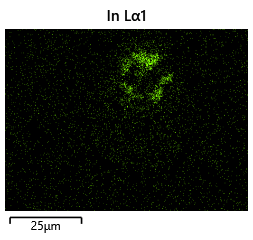
\includegraphics[height=1cm]{Main/Ch2/extracted/Indium/In-EP-EDx_TLED-01-A1-s2_media_image7.png} &
    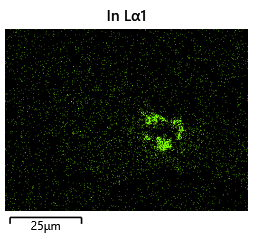
\includegraphics[height=1cm]{Main/Ch2/extracted/Indium/In-EP-EDx_TLED-01-A2-s1_media_image7.png} &
    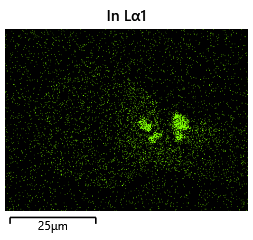
\includegraphics[height=1cm]{Main/Ch2/extracted/Indium/In-EP-EDx_TLED-01-A2-s2_media_image7.png} \\
    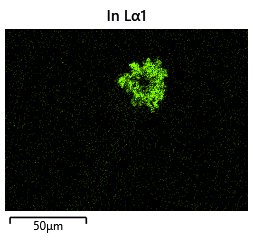
\includegraphics[height=1cm]{Main/Ch2/extracted/Indium/In-EP-EDx_TLED-01-B2-s1_media_image7.png} &
    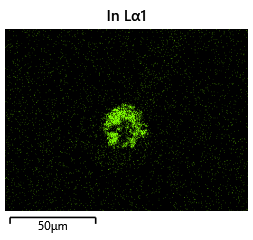
\includegraphics[height=1cm]{Main/Ch2/extracted/Indium/In-EP-EDx_TLED-01-B2-s2_media_image7.png} &
    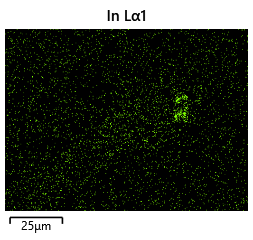
\includegraphics[height=1cm]{Main/Ch2/extracted/Indium/In-EP-EDx_TLED-02-A1-s1_media_image7.png} &
    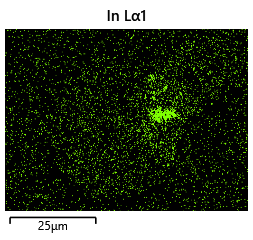
\includegraphics[height=1cm]{Main/Ch2/extracted/Indium/In-EP-EDx_TLED-02-A1-s2_media_image7.png} \\
    \includegraphics[height=1cm]{Main/Ch2/extracted/Indium/In-EP-EDx_TLED-02-A2-s1_media_image7.png} &
    \includegraphics[height=1cm]{Main/Ch2/extracted/Indium/In-EP-EDx_TLED-02-A2-s2_media_image7.png} &
    \includegraphics[height=1cm]{Main/Ch2/extracted/Indium/In-EP-EDx_TLED-02-B2-s1_media_image7.png} &
    \includegraphics[height=1cm]{Main/Ch2/extracted/Indium/In-EP-EDx_TLED-02-B2-s2_media_image7.png} \\
    \end{tabular}
    \caption{EDX Images of bonds, colour indicates presence of indium}
    \label{fig:EDX_indium_2}
\end{subfigure}
\caption{SEM and EDX images of the diebonds.}
\end{figure}


The results from the thermal simulations as seen in figure \ref{fig:thermal_simulations} in MATLAB were that there was more than sufficient time and heat to melt and wet the indium onto the opposing surface. As a result the lack of wetting was likely a result of one of the other issues (contaminants from the flip-chip process or some failure in the surface energies).
Both of the other issues are quite possible as during the process the substrate that is bonding onto the substrate with indium on the surface is face down on the `diebonder' which is an unclean surface that also does not have the appropriate surface energies and could dissipate the surface energy generated during the plasma cleaning process.
% TODO Verify statement about suface energy

It can be seen from the thermal simulations that the time taken for the indium to reach temperature is well within $0.3 \unit{\second}$ whereas the bonding recipe calls for the sample to sit at $250 \dC$ for $5 \unit{\minute}$. This is well within 2 orders of magnitude of time for the sample to reach temperature, as such it would be safe to assume that heat/temperature or lack thereof is not the causal source of failure.


\begin{figure}
    \centering
    \includegraphics[width=0.21\textwidth]{Main/Ch2/heat/001.png}
    \includegraphics[width=0.21\textwidth]{Main/Ch2/heat/002.png}
    \includegraphics[width=0.21\textwidth]{Main/Ch2/heat/008.png}
    \includegraphics[width=0.21\textwidth]{Main/Ch2/heat/020.png}
    \caption{Thermal simulation results. Temperature scale is ranged from $25 \dC$ to $250 \dC$}
    \label{fig:thermal_simulations}
\end{figure}


\section{Conformation to Theory}
In this section we wanted to ensure that there was uniform bonding across the area of the sample, this would arise from the bonding head providing relatively uniform bonding force over the sample area. From the microscope images in \ref{fig:microscopeIndium} we can see that the spread of the indium bumps is uniform over the area of the sample, this would be representative of the gimbal head providing relatively uniform pressure over the face of the sample.

Furthermore, we can also see that the bonding would spread according to the calculated volume.
To validate that the indium was spreading as expected, bumps were electroplated to achieve a width of $40 \um$. To achieve this we can use equation \ref{eq:radius_indium} where we conserve the volume of indium. We can assume that we can consistently generate indium bumps of width $h_{Initial} = 7\um$


\begin{equation} \label{eq:initial_radius}
    \begin{split}
        \sqrt{\frac{h_{Initial}}{ 0.65 \um}} r_{Initial} &= r_{Final} \\
        r_{Initial} &= \sqrt{\frac{h_{Initial}}{ 0.65 \um}}^{-1}r_{Final} \\
        r_{Initial} &= \sqrt{\frac{7 \um}{ 0.65 \um}}^{-1} 40 \um \\
        r_{Initial} &= 12 \um
    \end{split}
\end{equation}

The new GDS files for the altered indium bumps that should achieve a thickness of $40 \um$ looks like figure \ref{fig:12um_bumps_gds}.


\begin{figure}
    \centering
    \includegraphics[width=0.6\textwidth]{Main/Ch2/DC_DieBTest_V212um_tex_output.pdf}
    \caption{GDS file of electroplating sample with $12\um$ bumps. Green indicates the locations with indium electroplated. }
    \label{fig:12um_bumps_gds}
\end{figure}

After proceeding with the bonding the new images from the microscope look as follows in figure \ref{fig:12um_bumps_microscope}. The images look different as these samples were prepared for the following process in chapter \ref{sec:Ch3_elec}. However, the test for bonding performance is still relevant.


\begin{figure}
    \centering
    \def\w{0.35\textwidth}
    \begin{tabular}{cc}
        \includegraphics[width=\w]{Main/Ch2/12um/TL.png} &
        \includegraphics[width=\w]{Main/Ch2/12um/TR.png} \\
        \multicolumn{2}{c}{\includegraphics[width=\w]{Main/Ch2/12um/M.png}} \\
        \includegraphics[width=\w]{Main/Ch2/12um/BL.png} &
        \includegraphics[width=\w]{Main/Ch2/12um/BR.png}
    \end{tabular}
    \caption{Microscope images of diebonded $12 \um$ bumps.}
    \label{fig:12um_bumps_microscope}
\end{figure}

% insert image and reference to image


As can be clearly seen in the images that although there is some error in bonding spread, at this scale the placement accuracy limitations play a more significant role and constrain the critical dimension for the bond diameter. Furthermore, the bond size appears to conform to our expectations and reaches a size close to what was predicted.

While the size of the bonds deviate from the preliminary theory this is in part due to the basic modelling of the indium bumps that are assumed to be perfect cylinders. It is clear from the images taken with the SEM that this is not the case and both over plating and under plating cause serious decision from expected results \ref{fig:overplating}.

\begin{figure}
    \centering
    \begin{subfigure}[t]{0.3\textwidth}
        \includegraphics[width=\textwidth]{Main/Ch2/overplating/overplating.png}
        \caption{Microscope image of diebonding results from a sample that has been overplated}
    \end{subfigure}
    ~
    \begin{subfigure}[t]{0.3\textwidth}
        \includegraphics[width=\textwidth]{Main/Ch2/overplating/overplating-sem1.png}
        \caption{SEM image of electroplated bump from a sample that has been overplated}
        \label{fig:not-measured}
    \end{subfigure}
    ~
    \begin{subfigure}[t]{0.3\textwidth}
        \includegraphics[width=\textwidth]{Main/Ch2/overplating/overplating-sem2.png}
        \caption{SEM image of diebonding results from sample in \ref{fig:not-measured} (with measurements)}
    \end{subfigure}
    \caption{Images of sample that has been overplated.}
    \label{fig:overplating}
\end{figure}

While results seemed promising with the bonding the bonds from this series of experiments broke very easily. Many of the resulting bonds did not last long enough for the pick and place to remove the head and others failed to last long enough to be transported across the lab to the microscope for imaging of the bonds.
In the \ref{sec:bond_failures} I discuss the method by which the $\ch{AuIn2}$ bond forms and why failures occur.


\section{Bond failures}
\label{sec:bond_failures}

This section will complete a small literature review as to how the bond between the LED and BP forms and why there is failure in the previous experiments.

The \emph{Handbook of Wafer Bonding} \cite{waferBondingHandbook} suggests that a typical $\ch{In-Au}$ bump consists of a $3\um$ thick indium layer and a $0.3\um$ thick gold layer. The diagram in \ref{fig:waferbondingdiagram} part (a) shows what a typical construction of a microbump looks like. While there are differences in the way we construct our bond which looks like \ref{fig:bond_diagram}. The resulting product should be relatively similar.

\begin{figure}
    \definecolor{cadetgrey}{HTML}{91A3B0}
    \definecolor{chromeyellow}{HTML}{FFF600}
    \centering
    \begin{tikzpicture}
        \def\l{10cm}
        \def\t{12pt}

        \draw[draw=none, fill=CadetBlue!50] (0, 0) rectangle (\l, \t*3) node[midway] {Sapphire $\geq 400 \um$};
        \draw[draw=none, fill=cadetgrey!50] (0, \t*3) rectangle (\l, \t*4) node[midway] {$\ch{Cr} \approx 30 \nm$};
        \draw[draw=none, fill=chromeyellow!50] (0, \t*4) rectangle (\l, \t*5) node[midway] {$\ch{Au} \approx 200 \nm$};
        \draw[draw=none, fill=purple4!50] (\l*0.2, \t*5) rectangle (\l*0.7, \t*6) node[midway] {Photoresist $\approx 6-8 \um$ \cite{AZPdatasheet}};
        \draw[draw=none, fill=purple4!50] (\l*.95, \t*5) rectangle (\l, \t*6) ;
        \draw[draw=none, fill=purple4!50] (0, \t*5) rectangle (\l*.1, \t*6);
        \draw[draw=none, fill=cadetgrey!50] (\l*0.1, \t*5) rectangle (\l*.2, \t*6);
        \draw[draw=none, fill=cadetgrey!50] (\l*.7, \t*5) rectangle (\l*.95, \t*6) node[midway] {$\ch{In} \approx 6-8 \um$};

        \draw[draw=none, fill=CadetBlue!50] (0, \t*16) rectangle (\l/3, \t*19) node[midway] {Sapphire $\geq 400 \um$};
        \draw[draw=none, fill=cadetgrey!50] (0, \t*16) rectangle (\l/3, \t*15) node[midway] {$\ch{Cr} \approx 30 \nm$};
        \draw[draw=none, fill=chromeyellow!50] (0, \t*15) rectangle (\l/3, \t*14) node[midway] {$\ch{Au} \approx 200 \nm$};
        \node at (\l/2, \t*17.5) {Or};
        \draw[draw=none, fill=CadetBlue!50] (2*\l/3, \t*16) rectangle (\l, \t*19) node[midway] {Sapphire $\geq 400 \um$};
        \draw[draw=none, fill=cadetgrey!50] (2*\l/3, \t*16) rectangle (\l, \t*15) node[midway] {$\ch{Cr} \approx 30 \nm$};
        \draw[draw=none, fill=chromeyellow!50] (2*\l/3, \t*15) rectangle (\l, \t*14) node[midway] {$\ch{Au} \approx 200 \nm$ \cite{CrAuPresentation}};
        \draw[draw=none, fill=cadetgrey!50] (2*\l/3, \t*14) rectangle (\l, \t*13) node[midway] {$\ch{In} \approx 6-8 \um$};

    \end{tikzpicture}
    \caption{Bond diagram, photoresist is removed before diebonding.}
    \label{fig:bond_diagram}
\end{figure}


As described in the handbook.
\begin{quote}
    In addition, the  $\ch{Au - In}$ microbump has a relatively low yield strength, and thus undergoes plastic deformation under a mechanical load, which can help relieve mechanical stresses induced in the bonded wafers. The problems of thermal fatigue and creep movement due to the plastic deformation in the  $\ch{Au - In}$ microbumps can be mitigated by the epoxy adhesive surrounding them.

...

    As the temperature increases above $156\dC$, the molten indium dissolves the $\ch{AuIn2}$ intermetallic layer to form a mixture of indium - rich liquid with $\ch{AuIn2}$ grains. This liquid reacts with the remaining gold layer to form more $\ch{AuIn2}$ as shown in Figure \ref{fig:waferbondingdiagram}(c). Consequently, the composition of $\ch{AuIn2}$ in the mixture increases. During cooling to room temperature, the solidification of the mixture starts below $156\dC$ to form indium - rich $\ch{Au - In}$ alloys.
\end{quote}

Thus, the tensile strength of the alloy is comparable to that of $\ch{In}$ which has a tensile strength of $1.6 \mpa$ \cite{indiumCorpConstants} and a shear strength of $6.1 \mpa$.

Given that we have a bonded area of:


\begin{equation} \label{eq:bonded_area}
    \begin{split}
        A_{Bonded} &\doteq (6\times 6) \pi r^2 \\
        &= (6\times 6) \pi (20 \um)^2 \\
        &= 45239 \umm = 0.04524 \mm^2
    \end{split}
\end{equation}

The tensile strength is given by equation \ref{eq:tensile}.

\begin{equation} \label{eq:tensile}
    \begin{split}
        \sigma &= \frac{F_{tensile}}{A} \\
        1.6 \mpa \times A_{Bonded} &= F_{tensile} \\
        72.4 \unit{\milli\newton} &= F_{tensile}
    \end{split}
\end{equation}

The calculated tensile strength is extremely low, and the sheer strength is on a similar order of magnitude ($F_{shear} = 276 \unit{\milli\newton}$). This tensile and shear strength is only one order of magnitude greater than the mass of the LED and BP which are $M = \rho_{Sapphire} \times V_{LED + BP} = 0.21 \unit{\gram} \rightarrow F_{g} = M g = 2.1 \unit{\milli\newton}$. Due to the inaccuracies of the diebonder we do not observe 100\% overlap of the active bonding area which significantly reduces our margins required for maintaining a bond, furthermore the diebonder vacuum system has easily ripped the LED off of a bonded LED and BP pair with sub-nominal vacuum pressure.

Since the current setup fails very easily it requires a solution before we can proceed to the daisy-chain tests in the next chapter.
I explain in further detail in the following section how I approached how to resolve this issue.


\section{Development of a Repeatable Process}
\label{sec:Ch2_repeatable}

As previously described a number of bonds did not last long enough for the diebonder to remove the head from on top of the LEDs. While we expected the bonds to be mechanically insecure, we still expected them to handle careful transport for a few days while characterization could be done. Instead, we observed immediate failures. These failures could have been as a result of a variety of reasons, some of these reasons were described in the previous chapter. To avoid tautology the solutions discussed here were to improve the cleanliness of the handling of samples and to increase the bonded area that would bond the LED to the BP.

\subsection{Adding Anchors}

I wanted to add anchors to significantly improve the tensile strength of the bond. To complete this, inactive areas of the LED sample had portions where \uleds \ would not be placed where the $\ch{Cr}-\ch{Au}$ would not be etched away. Furthermore, on the BP those corresponding areas would have indium electroplated. The corresponding GDS file of the LED and BP look like \ref{fig:gds_bp_led_anchors}.



\begin{figure}
    \centering
    \includegraphics[width=0.6\textwidth]{Main/Ch2/DC_DieBTest_V5.GDStex_output.pdf}
    \caption{GDS file of LED and BP. Anchors added in alignment marks and between active areas. }
    \label{fig:gds_bp_led_anchors}
\end{figure}


The anchors in figure increase the bonding area by orders of magnitude while maintaining the functionality of the previous design.
The new area is \ref{eq:new_area}.


\begin{equation} \label{eq:new_area}
    \begin{split}
        A_{New} &\doteq \underbrace{(6\times 6) \pi r^2}_{\text{Area of bonds to LEDs}} \underbrace{((5\times 5) 260\um \times 40\um) + ((2\times 2 \times 4) 150\um \times 150 \um)}_{\text{Anchors}} \\
        &= (6\times 6) \pi (20 \um)^2  + 620000 \umm \\
        &= 665239 \umm = 0.6652 \mm^2
    \end{split}
\end{equation}

As the new bonded area is well over 14 times greater ($ \frac{A_{New}}{A_{Old}} = 14.704$) the corresponding tensile and shear strength should also scale accordingly.
As the purpose of this series of experiments is not to develop the strongest possible mechanical bonds between wafers, and the current solution was sufficient for our purposes. No further tests into the strength of bonds were conducted because the bonds held the samples together as seen in figure \ref{fig:anchored_samples}.


\begin{figure}
    \centering
        \includegraphics[width=0.45\textwidth]{Main/Ch2/anchors/TL.jpg}
        \includegraphics[width=0.45\textwidth]{Main/Ch2/anchors/TR.jpg}
        \includegraphics[width=0.45\textwidth]{Main/Ch2/anchors/BL.jpg}
        \includegraphics[width=0.45\textwidth]{Main/Ch2/anchors/BR.jpg}
    \caption{Microscope anchors of diebonding with anchors.}
    \label{fig:anchored_samples}
\end{figure}
